% N.B. : Assurez-vous de compiler ce fichier en employant "pdflatex" afin que les images soient incluses.

% Tout commentaire est bienvenu et devrait être adressé à "support@dms.umontreal.ca".

    % L'appel de \Requireackage{natbib} est fait dans dms.cls si \documentclass est appelé
    % avec l'option <natbib>.  Les options de <natbib> sont données ici.
    % Vous pouvez les modifier, p.ex. ajouter <round> si vous préférez des parenthèse (1) 
    % plutôt que des crochets [1].
\PassOptionsToPackage{longnamesfirst}{natbib}  
\documentclass[12pt,maitrise,frenchb,natbib,twoside,initial]{dms} 
% La commande précédente charge la classe "dms.cls" avec les options suivantes : 
%   -police de caractères en 12 pts 
%   -format adapté à une thèse de doctorat 
%   -écriture française (par défaut avec la classe)
%   -impression recto-verso.
%   -adapté pour le dépôt initial (enlever l'option pour le dépôt final)
%
% Modifiez cette commande selon vos besoin à l'aide des options suivants :
% maitrise			mémoire de maîtrise;
% phd				thèse de doctorat;
% phdart                        thèse de doctorat par articles;
% rapport			rapport de stage;
% travaildirige			travail dirigé;
% oneside			impression recto;
% twoside			impression recto-verso.
% initial			depot initial (sans l'option pour depot final)
% policeTNR                     pour utiliser (l'équivalent de) Times New Roman (sinon <lmodern> est chargé, la fonte par défaut)
% nobabel			document en anglais seulement
% frenchb			document en français
% frenchb,english		document contenant du français et de l'anglais (utiliser \selectlanguage{} )

\usepackage[utf8]{inputenc}	% Fait dans le classe		
\usepackage[T1]{fontenc}

% La commande \sloppy peut avoir des effets étranges sur les
% lignes de certains paragraphes.  Dans ce cas, essayez \fussy
% qui suppresse les effets de \sloppy. (\fussy est le comportement par défaut.)
% On redéfinit \sloppy, pour tenter de réduire les comportements étranges.  
% Le seul changement apporté à la version originale est la valeur de \tolerance.
\def\sloppy{%
  \tolerance 500%  %9999 dans LaTeX ordinaire, mauvaise idée.
  \emergencystretch 3em%
  \hfuzz .5\csname p@\endcsname
  \vfuzz\hfuzz}
\sloppy  

\usepackage[usenames,dvipsnames]{xcolor}
%\usepackage{courier}

\usepackage{graphicx,amsmath,amsfonts,amssymb,setspace,subfigure,color,icomma,dsfont}
% graphicx		Pour importer des images (PDF, JPG, PNG).
% amsmath		Écriture selon les normes de l'AMS.
% amsfonts		Fontes additionnelles de l'AMS.
% amssymb		Écriture des symbols de l'AMS.
% setspace		Permet de régler la distance interligne dans le document.
% subfigure		Simplifie l'inclusion de figures côtes-\`a-côtes.
% color			Pour l'utilisation de couleurs dans le texte.
% icomma		Reconnait la virgule comme caractère mathematique de facon intelligent
% dsfont		symboles mathématiques

\usepackage[pdfpagemode=UseNone,pdfstartview={XYZ null null null}]{hyperref}	% Cette extension permet l'insertion d'hyperliens dans votre document pdf.
 \definecolor{dark-red}{rgb}{0.4,0.15,0.15}					% Ici, trois couleurs sont définies et seront utilisées pour colorer les "hyperliens".
 \definecolor{dark-blue}{rgb}{0.15,0.15,0.4}
 \definecolor{medium-blue}{rgb}{0,0,0.5}
 \hypersetup{colorlinks,linkcolor={dark-red},citecolor={dark-blue},urlcolor={medium-blue}}
\usepackage{bookmark}  % Remédie à des petits problème de <hyperref> (important qu'il soit chargé après <hyperref>)
  % Enlever les commentaires et remplir cette section avec l'information pertinente.
  % Ceci ajoute des « méta-données » au pdf.  C'est optionnel, mais recommandé.
  % Vous pouvez voir ces méta-données en ouvrant un visionneur de pdf et en cherchant les
  % propriétés du pdf.  (Vous pouvez aussi tapez ' pdfinfo <nom-du-pdf> '  dans un terminal.)
  % Ces données sont utiles, par exemple, pour augmenter les chances qu'un algorithme de
  % recherche trouve votre document sur Internet, une fois diffusé.  Autrement dit, ceci
  % peut aider à augmenter la visibilité de votre travail.
%\hypersetup{
%    pdftitle = {Exemple d'une thèse}, 
%    pdfauthor = {Coadmin},
%    pdfsubject = {Exemple pour utiliser le gabarit du DMS},
%    pdfkeywords = {DMS, gabarit, exemple, thèse, mémoire, coadministrateur}
%}

% Numérotation des équations par section et numérotation des tableaux et figures par chapitre.
\numberwithin{equation}{section}
\numberwithin{table}{chapter}
\numberwithin{figure}{chapter}

% Définition des environnements utiles pour un mémoire scientifique.
% 1	%FR
\newtheorem{cor}{Corollaire}[section]
\newtheorem{deff}{Définition}[section]
\newtheorem{exemple}{Exemple}[section]
\newtheorem{lemme}{Lemme}[section]
\newtheorem{prop}{Proposition}[section]
\newtheorem{rem}{Remarque}[section]
\newtheorem{theo}{Théor\`eme}[section]

% Si vous préférez que les corollaires, definitions, théor\`emes, etc. soient numérotés par le même compteur, utilisez plutôt ce bloc de commandes : 
%2	% FR
%\newtheorem{corollary}{Corollaire}[section]
%\newtheorem{definition}[corollary]{Définition}
%\newtheorem{example}[corollary]{Exemple}
%\newtheorem{lemma}[corollary]{Lemme}
%\newtheorem{proposition}[corollary]{Proposition}
%\newtheorem{remark}[corollary]{Remarque}
%\newtheorem{theorem}[corollary]{Théor\`eme}

%Pour faire des énumérations : easylist
\usepackage[ampersand]{easylist}



\onehalfspacing				% Fixe la distance interligne \`a "1.5". Pour une interligne double, utilisez plutôt "\doublespacing".

\allowdisplaybreaks			% Cette commande autorise LaTeX \`a briser les blocs d'équations, permettant ainsi une couverture plus uniforme des pages.

%Commande pour numéroter les tableaux en chiffres romains (préfixe: le numéro du chapitre)
\renewcommand{\thetable}{\thechapter. \Roman{table}}

\setlength{\parskip}{1ex plus 3pt minus 1pt}

% Commandes pour linguistique
\usepackage{lng,lng-acro-fr}

% Commandes générales
\usepackage{gen}

% Feedback
\newcommand{\FL}[1]{\draft{\textbf{(FL)}}\footnote{\draft{#1}}}

%lstlistings for writing code in Python and XML
\usepackage{listings}
\usepackage{color}
\usepackage{setspace}
\definecolor{Code}{rgb}{0,0,0}
\definecolor{Decorators}{rgb}{0.5,0.5,0.5}
\definecolor{Numbers}{rgb}{0.5,0,0}
\definecolor{MatchingBrackets}{rgb}{0.25,0.5,0.5}
\definecolor{Keywords}{rgb}{0,0,1}
\definecolor{self}{rgb}{0,0,0}
\definecolor{Strings}{rgb}{0,0.63,0}
\definecolor{Comments}{rgb}{0.38, 0.25, 0.32}
\definecolor{Backquotes}{rgb}{0,0,0}
\definecolor{Classname}{rgb}{0,0,0}
\definecolor{FunctionName}{rgb}{0,0,0}
\definecolor{Operators}{rgb}{0,0,0}
\definecolor{Background}{rgb}{0.98,0.98,0.98}
\definecolor{gray}{rgb}{0.4,0.4,0.4}
\definecolor{darkblue}{rgb}{0.0,0.0,0.6}
\definecolor{cyan}{rgb}{0.0,0.6,0.6}
\lstdefinelanguage{Python}{
xleftmargin=1em,
framextopmargin=2em,
framexbottommargin=2em,
showspaces=false,
showtabs=false,
showstringspaces=false,
frame=l,
tabsize=4,
% Basic
basicstyle=\ttfamily\scriptsize\setstretch{1},
backgroundcolor=\color{Background},
% Comments
commentstyle=\color{Comments},
% Strings
stringstyle=\color{Strings},
% keywords
morekeywords={import,from,class,def,for,while,if,is,in,elif,else,not,and,or,print,break,continue,return,True,False,None,access,as,,del,except,exec,finally,global,import,lambda,pass,print,raise,try,assert},
keywordstyle={\color{Keywords}\bfseries},
% additional keywords
morekeywords={[2]@invariant,pylab,numpy,np,scipy},
keywordstyle={[2]\color{Decorators}\slshape},
emph={self},
emphstyle={\color{self}\slshape},
%
}
\linespread{1.3}

\lstdefinelanguage{XML}
{
  morestring=[b]",
  morestring=[s]{>}{<},
  morecomment=[s]{<?}{?>},
  stringstyle=\color{black},
  identifierstyle=\color{darkblue},
  keywordstyle=\color{cyan},
  morekeywords={xmlns,version,type}% list your attributes here
	numbers=left,
 numberstyle=\footnotesize,
 numbersep=1em,
 xleftmargin=1em,
 framextopmargin=2em,
 framexbottommargin=2em,
 showspaces=false,
 showtabs=false,
 showstringspaces=false,
 frame=l,
 tabsize=4,
% Basic
basicstyle=\ttfamily\scriptsize\setstretch{1},
backgroundcolor=\color{Background},
}

\newcommand{\mate}[4]{
  \begin{figure}[htb]
    (PG:) #2

    (PD:) #3

    (COND:) #4
  \caption{#1}
  \end{figure}
}

%%%%%%%%%%%%%%%%%%%%%%%%%%%%%%%%%%%%%%%%%%%%%%%%%%%%%%%
% ---------  D É B U T  D U  D O C U M E N T  ---------
%%%%%%%%%%%%%%%%%%%%%%%%%%%%%%%%%%%%%%%%%%%%%%%%%%%%%%%

\begin{document}

% La commande "\brouillon" imprime, au bas de chaque page, la date ainsi que l'heure de la derni\`ere compilation de votre fichier.
%\brouillon            

%!TEX root = memoire.tex

% Voici les variables pour la création de votre page titre.

\title{Intégration de VerbNet dans un réalisateur profond}
\author{Daniel Galarreta-Piquette}
\copyrightyear{2018}
\date{\today}									% Date de dépôt du document.
	% ces éléments ne doivent plus apparaittre selon les dierectives de la FESP
	% si toutefois vou souhaitez les inclure, il faudra aussi modifier le document dms.cls
% \president{Nom du président du jury}
% \directeur{Nom du directeur de recherche}
% \codirecteur{Nom du codirecteur}
% \membrejury{Nom du membre du jury} 
% \examinateur{Nom de l'examinateur externe}
% %\membresjury{ala, beta, gamma}
% %\plusmembresjury{psi, zeta, omega} 
% \repdoyen{Nom du représentant du doyen} 
\dateacceptation{Date d'acceptation}
\sujet{linguistique}							% Votre discipline de recherche, soit "mathématiques" ou "statistique".
%\orientation{mathématiques fondamentales}		% Cette commande est optionnelle. Les choix courants sont : "mathématiques fondamentales", "mathématiques de l'ingénieur" et "mathématiques appliquées".

\department{Département de traduction et linguistique}

% Fin des variables \`a définir. La commande "\maketitle" créera votre page titre.


\pagenumbering{roman}
\maketitle    
 

\chapter*{Sommaire} 	% La commande "\chapter*" crée un chapitre sans numéro, contrairement \`a la commande "\chapter" réguli\`ere.

% N.B. : La commande "\noindent" force LaTeX \`a ne pas indenter le nouveau paragraphe.
\noindent Ce mémoire explore les patrons de régime en anglais provenant de la ressource lexicographique \emph{VerbNet} et leur implémentation dans un système de génération automatique de texte.


\textbf{Mots-clés}: génération automatique de texte; réalisation linguistique; patrons de régime; cadres syntaxiques; verbes; Théorie Sens-Texte; traitement automatique des langues; linguistique

\chapter*{Summary}

\noindent blablabla

\textbf{Keywords}: natural language generation; linguistic realisation; government patterns; syntactic frames; Meaning-Text theory; linguistics; natural language processing
% TABLE DES MATIÈRES
\cleardoublepage
\pdfbookmark[chapter]{\contentsname}{toc}  %Crée un bouton sur la bar de navigation
\tableofcontents				% Table des mati\`eres.
% LISTE DES TABLEAUX
\cleardoublepage
\phantomsection
\listoftables
% LISTE DES FIGURES
\cleardoublepage
\phantomsection
\listoffigures	


%%%%%%%%%%%%%%%%%%%%%%%%%%%%%%%%%%%%%
%% LISTE DES SIGLES ET ABRÉVIATION %
%%%%%%%%%%%%%%%%%%%%%%%%%%%%%%%%%%%%%
%% Il est obligatoire, selon les directives de la FESP, 
%% pour une thèse ou un mémoire d'avoir une liste des sigles et 
%% des abréviations.  Si vous considérez que de telles listes ne seraient pas
%% pertinentes (si, par exemple, vous n'utilisez aucun sigle ou abré.), son
%% inclusion ou omission est laissé à votre discrétion.  En cas de doute,
%% parlez-en à votre directeur de recherche, le coadministrateur ou, ultimement, à
%% la FESP directement.
%%
%% Dans le cas où vous incluez une table des sigles et des abréviations,
%% vous pouvez enlever les % de la section suivante pour faire apparaître
%% un exemple d'une telle liste « fait à la main ».  Il existe des outils
%% plus sophistiqués si vous devez inclure une multitude de sigles et abréviations.
%% (Par exemple, le package <glossaries> peut faire des index élaborés.  Comme
%% son utilisation est technique, il n'y a pas d'exemple directement dans ce gabarit.
%% On invite les gens qui aurait à l'utiliser à consulter le wiki
%% du dms, le coadministrateur ou faire leur propre recherche.)

\chapter*{Liste des sigles et des abréviations}
\begingroup %Pour que le \renewcommand soit local
%Modifiez ce nombre (p.ex.remplacez 2 par 1.5) pour augmenter ou diminuer l'espace entre les lignes du tableau.
\renewcommand{\arraystretch}{2} 
\noindent\begin{tabular}{p{.2\textwidth} p{.7\textwidth}}
  GAT & Génération automatique de texte \\
  GP & Patron de régime, de l'anglais \textit{Government Pattern}\\
  DPOS  &  Partie du discours profonde, de l'anglais \textit{Deep Part of Speech}\\
  TST & Théorie Sens-Texte\\
  VN & \emph{VerbNet}\\
\end{tabular}
\endgroup  %Fin du groupe local pour \arraystretch



\chapter*{Remerciements}

Je voudrais d'abord adresser mes remerciements à mon directeur de mémoire, François Lareau, pour m'avoir guidé dans le développement de ce projet, puis pour m’avoir engagé sur son projet GenDR, financé par la subvention FRQSC 2016-NP-191042.

Je voudrais aussi remercier mes collègues de l’Observatoire Linguistique Sens-Texte pour les beaux midis passés à discuter et à rire, j'en garderai de très bons souvenirs.

Je tiens également à remercier ma famille pour m'avoir aidé financièrement et pour m'avoir cuisiné des repas. Finalement, tous mes amis qui m'ont encouragé, mais spécialement mes colocataires qui ont facilité mes dernières semaines de rédaction.

% Fin des pages liminaires. À partir d'ici, les premi\`eres pages des chapitres ne doivent pas être numérotées.

% Voici maintenant le chapitre d'introduction.
\NoChapterPageNumber 



%!TEX root = ../memoire.tex

\chapter*{Introduction}

% \noindent c'est mieux de changer la définition de \chapter et autres titres pour que ça soit uniforme

mémoire porte sur : implémentation de VN dans un générateur de texte
sous branche du TAl, qu'est-ce que la gat
la gat répond à quels besoins, quels domaines
Bref explicatoni de la structure de la gat
La réalisation linguistique

pour réaliser du texte le plus naturel possible, il faut se doter de ressource traitant les verbes
parler de la problématique
\draft{Parler de la problématique: Verbes sont les noyaux des énoncés, nous voulons implémenter une ressource de verbes dans un réalisateur profond pour élargir sa couverture. }

finalement objectif de ce mémoire, doter un réalisateur de ces données linguistiques grâce à VerbNet
TST, GenDR, héritier de MARQUIS. Nous commençons par l'anglais, mais comme c'est un réalisateur multilingue, on pourrait couvrir large pour d'autres langues comme il existe des variantes de VerbNet. utiliser python pour l'implémenter

Organisation du mémoire 6 chapitres:  parler de chacun





\pagenumbering{arabic}

% Ici débute le corps de votre texte.


%!TEX root = ../memoire.tex

\chapter{Extraction de l'architecture de\emph{Verbnet}}

Dans ce chapitre, nous verrons l'apport que la ressource lexicale \emph{VerbNet} peut offrir à des applications en traitement automatique du langage (TAL). Nous avons comme objectif d'extraire l'architecture de dictionnaire \emph{VerbNet} pour l'implémenter dans un dictionnaire de type sens-texte qui servira à générer du texte. Cet objectif provient d'une problématique que nous avions rencontré auparavant. Nous voulions savoir comment organiser notre dictionnaire en ce qui concernait les verbes. Car ceux-ci sont si riches et complexes qu'il nous fallait trouver un moyen systématique d'encoder cette partie du discours. De plus, il nous fallait l'encoder pour que notre nouveau dictionnaire puisse intéragir correctement avec les règles grammaticales du logiciel. En ce qui concerne les dictionnaires, parmi la communauté TAL,  il ne semble pas y avoir de consensus quant à la manière de procéder pour modéliser la classe verbale. La raison est simple,  les verbes démontrent des comportements variables, très riches au niveau de l'éventail de patrons de régime possibles pour un même verbe, et assez complexes ce qui nécessite beaucoup plus d'attention que d'autres parties du discours comme les noms qui démontrent beaucoup moins de variétés d'usage quant au nombre de patrons de régime. Ce qui fait en sorte que comme tous les verbes sont des prédicats, et que les prédicats sont les noyaux des énoncés, il faut les traiter avec soin, faute de quoi leur application en NLP sera médiocre. Cette problématique nous a donc amené à constater que VerbNet s'était penché sur ce problème et nous voulions vérifier si rouages de leur dictionnaire peuvent s'appliquer en génération automatique de texte. De nos jours, avec les modèles stochastiques où il n'y a pas d'analyse linguistique, on ne construit pas de dictionnaires ou de règles grammaticales, mais on le laisse le soin au système d'apprendre les règles par lui-même et de développer le lexique par lui-même en n'assignant pas de POS et en voyant les langues naturelles comme des suites de caractères. C'est une mode qui fonctionne présentement grâce à la quantité immense d'information qu'on retrouve et ces nouveaux corpus incroyables combinés avec la puissance des ordinateurs et l'apprentissage machine, certains font complètement fi de l'analyse linguistique dans leurs applications TAL. Toutefois, les utilités principales de ces systèmes sont de divers ordres de NLP, mais en en ce qui concerne la génération automatique de texte, le traitement de la langue se doit d'être impeccable \citep{lareau18}. D'où la nécessité de développer des outils puissant et rigoureux qui nécessiteront plus de temps à développer car il faudra créer les règles et enrichir le dictionnaire qui compose la langue. Pour ce faire, on doit recourir à des méthodes linguistiques qui étaient plus populaires dans la fin des années 90 et début 2000 (citer des systèmes). Toutefois, en étant bien conscient du changement de cap, nous pensons qu'il est encore primordial de développer de bons outils linguistiques computationnels car c'est de cette manière qu'on pourra le mieux représenter le fonctionnement de la langue. De plus, nombres de chercheurs combinent l'apprentissage machine à des règles et des dictionnaires pour ainsi développer le lexique partiellement en annotant automatiquement des lexèmes.(trouver une citation dans les INLG de 2014 à 2017)

\section{VerbNet}

Ainsi, tel que mentionné précédemment, VerbNet a été créé dans un contexte où il y avait un réel besoin de réfléchir à la meilleure manière de procéder pour construire un dictionnaire qui saura tenir compte de la richesse et la complexité que renferment les verbes \citep{KipperClassBasedConstructionVerb2000}. C'était en réponse au manque de lignes directrices sur l'organisation des verbes dans les dictionnaires destinés à des applications TAL et ce malgré la quantité impressionnante de dictionnaire computationnels existants déjà. Parmi ceux qui ont tenté la chose, nous nommerons : le generative lexicon de Pustojevsky \citep{PustejovskyGenerativeLexicon1991} WordNet de Fillmore \citep{MillerWordNetLexicalDatabase1995}, ComLex\citep{Grishman:1994:CSB:991886.991931}, LCS\citep{13776} et FrameNet\citep{BakerBerkeleyFrameNetProject1998}. Ceux-ci comportaient des lacunes que du point de vue du traitement des entrées lexicales verbales, selon les auteurs de VerbNet. Les lacunes étaient diverses mais importantes, par exemple, ils trouvaient que le Generative Lexicon ne focusait que sur les noms, que WordNet ne donnait pas de détails concernant les cadres syntaxiques possibles  et aucune mention de la structure prédicat-argument. Quant à ComLex, ils décrivaient effectivement les cadres syntaxiques possibles, mais ne faisait pas de désambiguisation sémantique. Finalement, ils jugeaient que le lexicon LCS a essayé de palier à ces lacunes aussi, mais l'étentue lexicale qu'il offrait n'était pas assez large à leur goût\citep{SchulerVerbnetBroadcoverageComprehensive2005}. C'est donc dans ce contexte qu'est né le projet VerbNet.

\subsection{Levin et l'organisation en classes verbales}

Levin a bâti un lexicon verbal de l'anglais. Ses recherches portaient sur les propriétés sémantiques et syntaxiques des verbes. Selon elle, les composantes sémantiques des verbes déterminent  la manière dont ils se combinent avec leurs arguments. Elle a tenté de répertorié et systématiser les divers cadres syntaxiques des verbes. Puisque les verbes forment les noyaux des énoncés et qu'ils sont prédicats, Levin y a vu un intérêt académique. De plus, les verbes démontrent des propriétés extrêmement complexes contrairement aux autres prédicats se trouvant dans les autres PDD. Il existe un éventail de combinaisons possibles pour un verbe avec ses arguments et tout locuteur natif d'une langue sait quels sont les diathèses possibles et les arguments possibles pour un verbe. Et ce, sans avoir de connaissances linguistiques au prébalable, il s'agit d'une intuition de locuteur natif. Pour cette raison, Levin voulait regrouper les verbes en classes verbales en se basant sur son intuition de locutrice native. Ainsi, en testant divers patrons de régime des groupes de verbes, elle a délimiter un nombre impressionnant de classes verbales où chaque verbe compris dans cette classe partage des cadres syntaxiques avec les autres membres de sa classe.

Tel que Levin le dit \citep{verb-classes.levin.1993}, son travail a été guidé par l'idée que les comportements syntaxiques des verbes sont motivés par les composantes sémantiques qui les représente. À ces fins, Levin a observé les comportements des verbes en anglais pour y tester cette hypothèse linguistique car il pensait que c'était une bonne manière de démontrer la chose. Si des verbes qui partagent le même type de comportement syntaxique, ils doivent aussi probablement partager des caractéristiques sémantiques. Son travail a été de classer les verbes systématiquement. Déjà , Levin soulignait l'importance d'encadrer les verbes dans les lexicons car les verbes qui sélectionne des arguments démontrent un ensemble complexes de propriétés. Ainsi, au lieu de construire un dictionnaire où chaque entrée verbale est prise individuellement, on regroupe les entrées lexicales en classe en fonction de leur comportement syntaxique et sémantique. 

À la base le traitement est fait en fonction du comportement syntaxique, puis selon Levin, les verbes qui partagent le même type d'alternations syntaxiques (patrons de régime) partagent aussi la sémantique sous-jacente à ces constructions, donc cela fait en sorte qu'ils partagent généralement les mêmes caractéristiques sémantiques aussi. Le fait d'organiser le dictionnaire en classe verbale accélère le processus de création du dictionnaire, car une fois qu'on détermine le nombre de verbes qui fonctionnent de la même manière, il ne reste plus qu'à faire une entrée qui retient l'information syntaxique et sémantique partagée par l'ensemble de la classe, et passer à la classe suivante. Après, lorsqu'on a fait le tour des verbes, on a juste à les ajouter à l'une des classes pré-existantes. Les créateurs de VerbNet sont conscients du fait qu'on va parfois tenter de faire rentrer un verbe dans une classe et que c'est un brin tirer par les cheveux, mais il s'agit d'une infime partie du dictionnaire. \citep{SchulerVerbnetBroadcoverageComprehensive2005}. 

Ici, on voit que les verbes spray/load peuvent exprimer leurs arguments d'au moins deux manières différentes. La seconde manière que Levin a appelé "locative alternation".

\ex. \label{spray} Cadre syntaxique : Spray
	\a. Sharon sprayed water on the plants.
	\b. Sharon sprayed the plants with water.
	
\ex. \label{load} Cadre syntaxique : Load
	\a. The farmer loaded apples into the cart.
	\b. The farmer loaded the cart with apples.
	
Ces mêmes locuteurs natifs savent que des verbes qui s'apparentent à Spray/Load (car ils semblent correspondre au même type d'évènement) ne permettent pas les 2 alternances démontrées en \ref{spray} et en \ref{load}. Les verbes fill/cover permettent l'option b) et les verbes dump/pour permettent l'option a). Ainsi, à partir de tests de ce type, pour voir quels verbes permettaient le même type de construction, elle a bâti un lexicon qui regroupe les verbes en fonctions des alternances  de diathèses qu'ils permettent.
	
\ex. \label{cover} Alternances de diathèses : cover
	\a. * Monica covered a blanked over the baby.
	\b. Monica covered the baby with a blanket.

\ex. \label{fill} Alternances de diathèses : fill
	\a.* Gina filled lemonade into the pitcher. 
	\b. Gina filled the pitcher with lemonade. 

\ex. \label{pour} alternances de diathèses : pour
	\a. Carla poured lemonade into the pitcher. 
	\b. * Carla poured the pitcher with lemonade

\ex. \label{dump} alternances de diathèses : dump
	\a. The farmer dumped apples into the cart. 
	\b. *The farmer dumped the cart with apples. 
	
On en vient ainsi à la conclusion, que ces verbes ont beau ressembler à Spray/Load, mais il ne permettent pas les mêmes cadres syntaxiques, donc il y a une composante sémantique qui fait défaut et on ne peut pas avoir les mêmes frames. Ainsi, en opposant diverses diathèses possibles, Levin a fait un travail collossal où elle a repertorié des verbes se combinant de la même manière. C'est pourquoi des verbes qui ont beau être des synonymes, ne se combinent pas de la même manière. Elle avait ainsi un éventail de diathèses à tester et elle regroupait en classe les verbes qui partagaient les mêmes alternances. Se justifiant ainsi en disant que les raisons qui sous-tendent un partage des diathèses proviennent d'une sémantique similaire. 


Remettre l'exemple de VerbNet (plus clair) :

(cette partie manque l'exemple venant de verbnet)Ainsi, tel que démontré en \ref{transitive} et \ref{middle} les verbes appartenant à la classe break et à la classe cut se ressemblent car ils peuvent tous les 2 prendre ces cadres syntaxiques (ce genre de construction syntaxique). Toutefois, en \ref{intransitive} et en \ref{conative}, on voit très bien qu'il ne partagent pas ces constructions syntaxiques. \emph{Break} prend seulement la construction intransitive et exclut l'autre, tandis que \emph{cut} prend la construction conative et exclut l'intransitive. La raison que Levin donne est la suivante. Le verbe \emph{cut} décrit une série d'actions ciblant la complétion d'un but (séparer un objet en morceau). Toutefois, il est possible de faire ces séries d'actions sans que l'objectif final ne soit atteint, mais l'action de couper peut quand même être perçue. En ce qui concerne \emph{break}, la seule chose qui importe dans l'évènement, c'est le changement d'état d'un objet (qui devient séparés en morceaux). Si on n'arrive pas au résultat, une tentavive de briser quelque chose ne peut être perçue. Ce qu'on peut tirer de cet exemple, est que les classes verbales regroupent des verbes qui partagent des comportements syntaxiques similaires, les membres des classes ne sont donc pas nécessairement des synonymes, il ne s'agit que de verbes qui s'utilisent de la même façon. Ainsi, certaines classes vont effectivement regrouper des verbes qui signifient à peu près la même chose, mais aussi des verbes qui en surface, ne partagent pas bcp avec une majorité des verbes de cette classe, mais syntaxiquement, ces membres se comportent comme le reste de la classe. Ainsi, selon Levin, il y a quelque chose derrière les composantes sémantiques de ces membres qui les unirait avec les autres qui se ressemblent.

Ainsi, les créateurs de VerbNet ont repris les concepts de Levin, mais les ont retravaillé. Toutefois, l'idée de constuire le lexicon verbal en classes est directement hérité de Levin.  L'orgaisation hiérarchique est aussi directement inspiré de la hiérarchie que Levin avait pensé. Toutefois,VerbNet a aussi ajouté des classes à ce que Levin avait fait. Ce qu'ils appellent intersective Levin classes, ce sont des sous-ensembles de classes qui s'entrecoupent et forment des classes à part. \citep{SchulerVerbnetBroadcoverageComprehensive2005}et \citep{verbnet.2006}.

\subsection {Composantes de VerbNet}  

VerbNet est composé de classes verbales. Chaque classe contient un ensemble de membres, une liste de rôles thématiques (accompagnés de restrictions) utilisés pour les cadres syntaxiques et sémantiques, puis un ensemble de cadres possibles pour une classe. Chaque cadre est composé d'une brève description, d'un exemple, d'une description syntaxique et d'un ensemble de prédicats décrivant le cadre\citep{SchulerVerbnetBroadcoverageComprehensive2005}.

\subsubsection{Classes verbales : organisation hiérarchique}

Les raisons qui ont motivé VerbNet a organisé son information en hiérarchie. D'abord, il se sont fortement inspiré de Acquilex Lexical Knowledge Base \citep{CopestakeACQUILEXLKBrepresentation1992}. Ensuite, pour des raisons pratiques, ils ont trouvé que c'était la meilleure manière d'organiser cette montagne d'information lexicale car ils ont revu l'information fournie par Levin et ont ajouté des sous-classes aux classes ainsi que des sous-sous-classes aux sous-classes, allant jusqu'à un niveau de 3 steps de profondeur. Donc, des sous-ensembles des sous-ensembles. Ce qu'ils considèrent comme une raffinement des classes originales de Levin \citep{SchulerVerbnetBroadcoverageComprehensive2005}. En gros, c'est l'ajout de sous-classes aux classes origniales de Levin (et aux sous-sous-classes) qui ont rendu VerbNet hiérarchique. 

Le fonctionnement est assez simple. Une sous-classe fille hérite de toute l'information de sa classe mère. Les sous-classes sont à l'origine de vouloir spécifier le comportement qui rassemble un sous-ensemble des membres d'une classe. Ainsi, une sous-classe est un ajout d'information par rapport à des restrictions d'usages de rôles thématiques, de cadres syntaxiques ou de prédicats sémantiques.(guidelines, \citep{SchulerVerbnetBroadcoverageComprehensive2005})

Par la suite, on se sert encore de la numérotation pour expliciter la hiérarchie à l'intérieur même d'une classe (guidelines). Chaque classe peut inclure des classes filles, qui sont des classes sœurs entre elles, et qui peuvent avoir des classes filles à leur tour. La classe verbale Spray en démontre bien la chose. 

D'abord, il y a la classe supérieure, qui est la plus haute de la hiérarchie, toutes les caractéristiques de cette classe sont partagées par tous les verbes de la classe. Dans la top classe nous avons les constructions syntaxiques et les prédicats sémantiques partagés par la classe, ainsi que les rôles thématiques. 

Une classe mère domine une sous-classe, toutes ses caractéristiques sont partagées avec les classes subordonnées à celle-ci. 

Une sous-classe : Les sous-classes dans VerbNet héritent des caractéristiques provenant de la classe dominante, mais elles spécifient particulièrement des constructions syntaxiques et une sémantique entre les verbes membres de cette sous-classe. Ce qui est spécifié dans une sous-classe peut être de différents ordres : ajouter des constructions syntaxiques propres à ce sous-groupe, ajouter des restrictions sélectionnelles sur les étiquettes des rôles sémantiques. 

Des classes sœurs, ne partagent pas de caractéristiques hormis celle héritées par leur classe mère. Le reste de l'information encodée dans la classes sœurs n'est valide qu'à l'intérieur de leur classe respectivement.

Démontrer la chose comme dans Guidelines :

\begin{easylist}[itemize]
& Spray-9.7
&& Spray-9.7-1
&&& Spray-9.7-1-1
&& Spray-9.7-2
\end{easylist}

Les classes verbales de VerbNet sont numérotées par des chiffres allant de 9-109 (guidelines). Le système de numérotation est directement hérité de Levin \citep{verb-classes.levin.1993} Ainsi, le numéro apparaissant devant une classe verbale est associé à des caractéristiques sémantiques et syntaxiques communes. Par Exemple, les classes verbales associées à des verbes de type "mettre quelque chose" commenceront par le chiffre 9. Ce qui nous donne quelque chose comme : 

\begin{easylist}[itemize]
  & put 9.1
	& put spatial 9.2
	& funnel 9.3
	& put direction 9.4
	& pour 9.5
	& coil 9.6
	& spray 9.7
	& fill 9.8
	& butter 9.9
	& pocket 9.10
	
\end{easylist}

Certains numéros n'impliquent qu'une seule classe, car il n'y a pas d'autres classes qui partagent ce genre de traits sémantiques ou syntaxiques communs.

\subsubsection{Membres}

L'ensemble des membres d'une classe :
\begin{lstlisting}[language=XML, caption = les membres]
<VNCLASS ID="give-13.1" xmlns:xsi="http://www.w3.org/2001/XMLSchema-instance" xsi:noNamespaceSchemaLocation="vn_schema-3.xsd">
    <MEMBERS>
        <MEMBER name="deal" wn="deal%2:40:01 deal%2:40:02 deal%2:40:07 deal%2:40:06" grouping="deal.04"/>
        <MEMBER name="lend" wn="lend%2:40:00" grouping="lend.02"/>
        <MEMBER name="loan" wn="loan%2:40:00" grouping=""/>
        <MEMBER name="pass" wn="pass%2:40:00 pass%2:40:01 pass%2:40:13 pass%2:38:04" grouping="pass.04"/>
        <MEMBER name="peddle" wn="peddle%2:40:00" grouping="peddle.01"/>
        <MEMBER name="refund" wn="refund%2:40:00" grouping="refund.01"/>
        <MEMBER name="render" wn="render%2:40:02 render%2:40:01 render%2:40:00 render%2:40:03" grouping="render.02"/>
        <!--removed "trade" from class because doesn't take "to-PP"-->
        <!--removed "volunteer "from class because doesn't fit dative or-->
        <!--PP recipient PP frames-->
    </MEMBERS>
\end{lstlisting}

\subsubsection{Rôles thématiques}

(ce que je veux, ce sont des beamer arrows qui permettent de pointer vers qqch à l'intérieur de listings, tikz style)

VerbNet utilise un ensemble de 23 rôles thématiques pour identifier les arguments dans les classes verbales (vérifier de quels rôles thématiques ils s'inspirent).On étiquette les arguments dans les classes verbales en leur associant un rôle thématique. La raison pour laquelle VerbNet a opté pour les rôles thématiques est que, contrairement à un étiquetage générique où on énumère les arguments en procédant comme "Argument 1" Verbe "Argument 2" pour illustrer un cadre syntaxique est parce que les rôles thématiques peuvent offrir de l'information sémantique de plus que juste un argument numéroté. Effectivement, à la base, les rôles thématiques ont été pensés dans les années 60 pour assigner une fonction aux arguments sélectionnés par des prédicats. On les avait créé pour typer les participants des prédicats. La spécification du rôle fournit de l'information sémantique sur le type d'argument en jeu, tandis que numéroté ne fournit rien du tout. Chaque argument se fait donné un rôle thématique unique, et ces rôles thématiques sont partagés par tous les membres d'une classe. Donc, ils doivent être assez large pour que ce soit cohérent avec tous les membres, mais pas trop imprécis non plus. Les rôles thématiques correspondent à la relation sémantique qui existe entre un prédicat et ses arguments.

VerbNet utilise les rôles thématiques pour étiquetter les arguments figurant des les cadres syntaxiques (et sémantiques) (Schuler, 2005). Elle puise dans une banque de 23 rôles thématiques pour associer le bon rôle à l'argument en question. Ils ont choisi ces rôles car ils étaient assez généraux pour se prêter à toutes les évènements que dégagent les verbes dans le dictionnaire. Ils voulaient capturer l'essence des verbes et démontrer encore une fois le caractère général des verbes en démontrant qu'une poignée d'argument peut bel et bien rendre compte des arguments sélectionnés par les verbes en anglais. À l'intérieur d'une même classe verbale on y retrouve un nombre x de rôles thématiques qui seront mappés aux arguments sélectionnés dans les cadres syntaxiques et sémantiques fournis par VerbNet. Ils ont choisi les rôles thématiques au lieu d'autres moyens d'étiquettage des arguments car ils trouvaient que ça ajoutait de l'information sémantique sur une classe verbale. 

Les rôles thématiques choisis par VerbNet sont de divers ordres, certains proviennent des premiers pensés par (Fillmore,1968) d'autres de Jackendoff (Jackendoff, 1972), et des ajouts pour compenser pour les classes qui nécessiteraient des rôles plus spécifiques à leur classes, tout en étant assez généraux pour pouvoir se prêter à d'autres classes. Encore une fois, tel que mentionné dans le background de Dissertation, certains critiques les rôles thématiques car ils ont un caractère assez arbitraires et il n'est pas facile de tout justifier. De cette manière, les rôles thématiques utilisés par VerbNet n'ont pas été créé systématiquement, mais plus en fonction de ce qui cadrait le plus avec les classes verbales et les arguments nécessaires qui apporteraient le plus d'information sémantique pertinente. Ils ne pensent pas qu'un ensemble plus petits de rôles thématiques aurait pu être suffisant, mais ils ne pensent pas non plus que ceux qu'ils ont choisi sont exactement ce dont on aurait besoin, il n'ont pas nécessairment été au bout de tous les rôles thématiques possibles. Mais, ils considèrent que ce qu'ils avaient était suffisant pour rendre compte des comporetements des arguments envers leur prédicats respectifs, et ce pour toutes les classes verbales.

À l'intérieur d'une classe verbale (ou sous-classe, etc.), chaque argument se fait assigner un rôle thématique

Les rôles thématiques nous donne de l'information sur la sémantique des participants d'une phrase dans le but que les différents cadres syntaxiques (alternances) n'influencent pas les rôles assignés. On nous fourni un exemple que nous réutiliserons pour illustrer le propos (guidelines) :

\ex. \label{semantic roles}
	\a. Sandy shattered the glass.
	\b. The glass shattered

D'un point de vue de la syntaxe, dans la première phrase, Sandy est le sujet du verbe et the glass en est l'objet direct. Tandis que dans la seconde phrase, the glass est le sujet du même verbe, et il n'y a pas d'objets directs. En leur assignant un rôle thématique, on notera que d'un point de vue de la sémantique rien n'a changé, même si la structure a changé en apparence. Ainsi, si on assigne un rôle d'Agent à Sandy et un rôle de Patient à the glass, on remarque que les rôles sémantiques sont cohérents avec la phrase, malgré le changement de sujet et d'objet direct.

Les rôles thématiques sont explicités au début d'une classe verbale. (exemples venant de break-45.1.xml) 
%de la documentation de VerbNet: http://verbs.colorado.edu/verbnet_downloads/downloads.html

\begin{lstlisting}[language=XML, caption = les rôles thématiques]
    <THEMROLES>
        <THEMROLE type="Agent">
            <SELRESTRS logic="or">
                <SELRESTR Value="+" type="animate"/>
                <SELRESTR Value="+" type="organization"/>
            </SELRESTRS>
        </THEMROLE>
        <THEMROLE type="Theme">
            <SELRESTRS/>
        </THEMROLE>
        <THEMROLE type="Recipient">
            <SELRESTRS logic="or">
                <SELRESTR Value="+" type="animate"/>
                <SELRESTR Value="+" type="organization"/>
            </SELRESTRS>
        </THEMROLE>
    </THEMROLES>
\end{lstlisting}
Finalement, les rôles thématiques sont domain-general, voulant dire qu'on veut les réutiliser dans le plus de classes là où c'est pertinent. Ils ne sont pas spécifiques à une classe ou un verbe, on les retrouve partout dans le lexicon. C'est pourquoi on veut qu'ils soient assez général pour rendre compte de divers type d'arguments.

Pour les besoins de notre travail, nous n'utilisons pas les rôles thématiques dans notre travail, mais nous voulions souligner qu'ils étaient importants pour les créateurs de VerbNet. 
Voir les raisons de Melcuk p.230

\subsubsection{Restrictions sélectionnelles}

Les restriction sélectionnelles vont sur les rôles thématiques. Est-ce que c'est pertinent d'en parler ? Probablement, pas, on ne s'en sert pas du tout.
En gros, il s'agit de restrictions imposées aux rôles thématiques pour que ça sélectionne un certain type d'argument. Ainsi, parmi ces restrictions, parfois, certains verbes requièrent que l'Agent soit nécessairement de type x, tandis que le patient peut être n'importe quoi. OU l'inverse, etc.
Ça donne encore plus d'informations sur le participant de la phrase, de plus, VerbNet considère que ces restrictions sélectionnelles offrent encore plus d'information sémantique, car on précise le type d'argument requis.
\begin{lstlisting}[language=Xml, caption = les restrictions sélectionnelles]
    <THEMROLES>
        <THEMROLE type="Agent">
            <SELRESTRS logic="or">
                <SELRESTR Value="+" type="animate"/>
                <SELRESTR Value="+" type="organization"/>
            </SELRESTRS>
        </THEMROLE>
        <THEMROLE type="Theme">
            <SELRESTRS/>
        </THEMROLE>
        <THEMROLE type="Recipient">
            <SELRESTRS logic="or">
                <SELRESTR Value="+" type="animate"/>
                <SELRESTR Value="+" type="organization"/>
            </SELRESTRS>
        </THEMROLE>
    </THEMROLES>
\end{lstlisting}

\subsubsection{Cadres syntaxiques}

Pour une classe donnée, on y retrouve soit un ou des cadres syntaxiques qui servent à représenter le type de réalisation de surface possible pour cette classe verbale. D'ailleurs, ces cadres syntaxiques sont partagés par l'ensemble des membres d'une classe ou d'une sous-classe. Chaque cadre syntaxique décrit une construction verbale de type transitives directes/indirectes, des intransitives, des phrases prépositionnelles, etc. Un cadre syntaxique est composé de rôles thématiques dans leur position argumentale ainsi que le verbe qui les régie (ainsi que d'autres unités lexicales nécessaires au bon fonctionnement d'une construction).

À l'intérieur de chaque classe verbale, on retrouve la liste des membres, suivie de la liste des rôles thématiques qu'on retrouve dans les cadres syntaxiques de cette classe, puis les cadres syntaxiques. Ainsi, on liste tous les cadres syntaxiques possibles pour une classe. Ce qui nous donne de l'information de nature syntaxique et explicite les liens qui unissent les rôles thématiques au verbe en question. Ça nous donne aussi beaucoup d'information concernant le verbe, car on voit comment il peut être utilisé, quel genre d'actant il sélectionne, de quel type de patron de régime il s'agit. C'est ce qui nous intéresse le plus à la base. C'est de savoir comment ce verbe se combine, peut-il prendre un verbe comme complément d'objet direct, est-ce qu'il sélectionne telle ou telle préposition. Bref, l'information contenue dans les cadres syntaxiques est très pertinente pour notre travail, car il existe très peu de dictionnaires qui ont voulu énumérer toutes les alternances syntaxiques d'un verbe. Puis, les cadres syntaxiques respectent aussi la caractéristiques hiérarchique omniprésente dans VerbNet. Ainsi, tous les membres d'une classe partagent ces patrons de régime, et une sous-classe hérite aussi des patrons de régime de la classe qui la gouverne. 

guidelines: Les cadres syntaxiques sont compris dans la section FRAMES de VerbNet qui contient, les cadres syntaxiques ainsi que les prédicats sémantiques. Cela nous donne une description des différentes réalisation en syntaxe de surface et des alternances de diathèses permises pour les verbes représentés par cette classe. On a ainsi une vue d'ensemble sur les constructions syntaxiques possibles par classe verbale. 

Dans la figure ci-bas, on voit le début de FRAMES, qui est la balise comprenant tous les FRAME qui eux sont des cadres. À l'intérieur de FRAME, on a SYNTAX et SEMANTICS. Commençons d'abord par SYNTAX, et faisons abstraction de DESCRIPTION et EXAMPLES pour l'instant.

\begin{lstlisting}[language=Xml, caption = cadres syntaxiques]

            <SYNTAX>
                <NP value="Agent">
                    <SYNRESTRS/>
                </NP>
                <VERB/>
                <NP value="Theme">
                    <SYNRESTRS/>
                </NP>
                <PREP value="to">
                    <SELRESTRS/>
                </PREP>
                <NP value="Recipient">
                    <SYNRESTRS/>
                </NP>
            </SYNTAX>
\end{lstlisting}

\subsubsection{Prédicats sémantiques}

VerbNet est fier de pouvoir offrir de l'information sémantique en plus d'information syntaxique. Voici comment ils mettent leur information sémantique.
Les prédicats sémantiques = dénoter les relations entre participants d'un évènement et l'évènement en soi. Ils sont utilisés pour transmettre les key components of meaning d'une classe verbale.

Dissertation : Les prédicats sémantiques sont utilisés pour véhiculer des composantes sémantiques importantes de chaque classe verbale. Ces prédicats sémantiques dénotent les relations entre les participants et les évènements. Dans verbnet, l'information sémantique est exprimée par une conjonction de prédicats sémantiques. Ces prédicats sémantiques peuvent ...

\begin{lstlisting}[language=Xml, caption=Les prédicats sémantiques]
<SEMANTICS>
                <PRED value="has_possession">
                    <ARGS>
                        <ARG type="Event" value="start(E)"/>
                        <ARG type="ThemRole" value="Agent"/>
                        <ARG type="ThemRole" value="Theme"/>
                    </ARGS>
                </PRED>
                <PRED value="has_possession">
                    <ARGS>
                        <ARG type="Event" value="end(E)"/>
                        <ARG type="ThemRole" value="Recipient"/>
                        <ARG type="ThemRole" value="Theme"/>
                    </ARGS>
                </PRED>
                <PRED value="transfer">
                    <ARGS>
                        <ARG type="Event" value="during(E)"/>
                        <ARG type="ThemRole" value="Theme"/>
                    </ARGS>
                </PRED>
                <PRED value="cause">
                    <ARGS>
                        <ARG type="ThemRole" value="Agent"/>
                        <ARG type="Event" value="E"/>
                    </ARGS>
                </PRED>
            </SEMANTICS>
\end{lstlisting}

Pour mieux exposer leur sémantique, nous avons fait un tableau qui exemplifie les prédicats sémantiques pour l'énoncé : give
\begin{figure}[h]
	\centering
	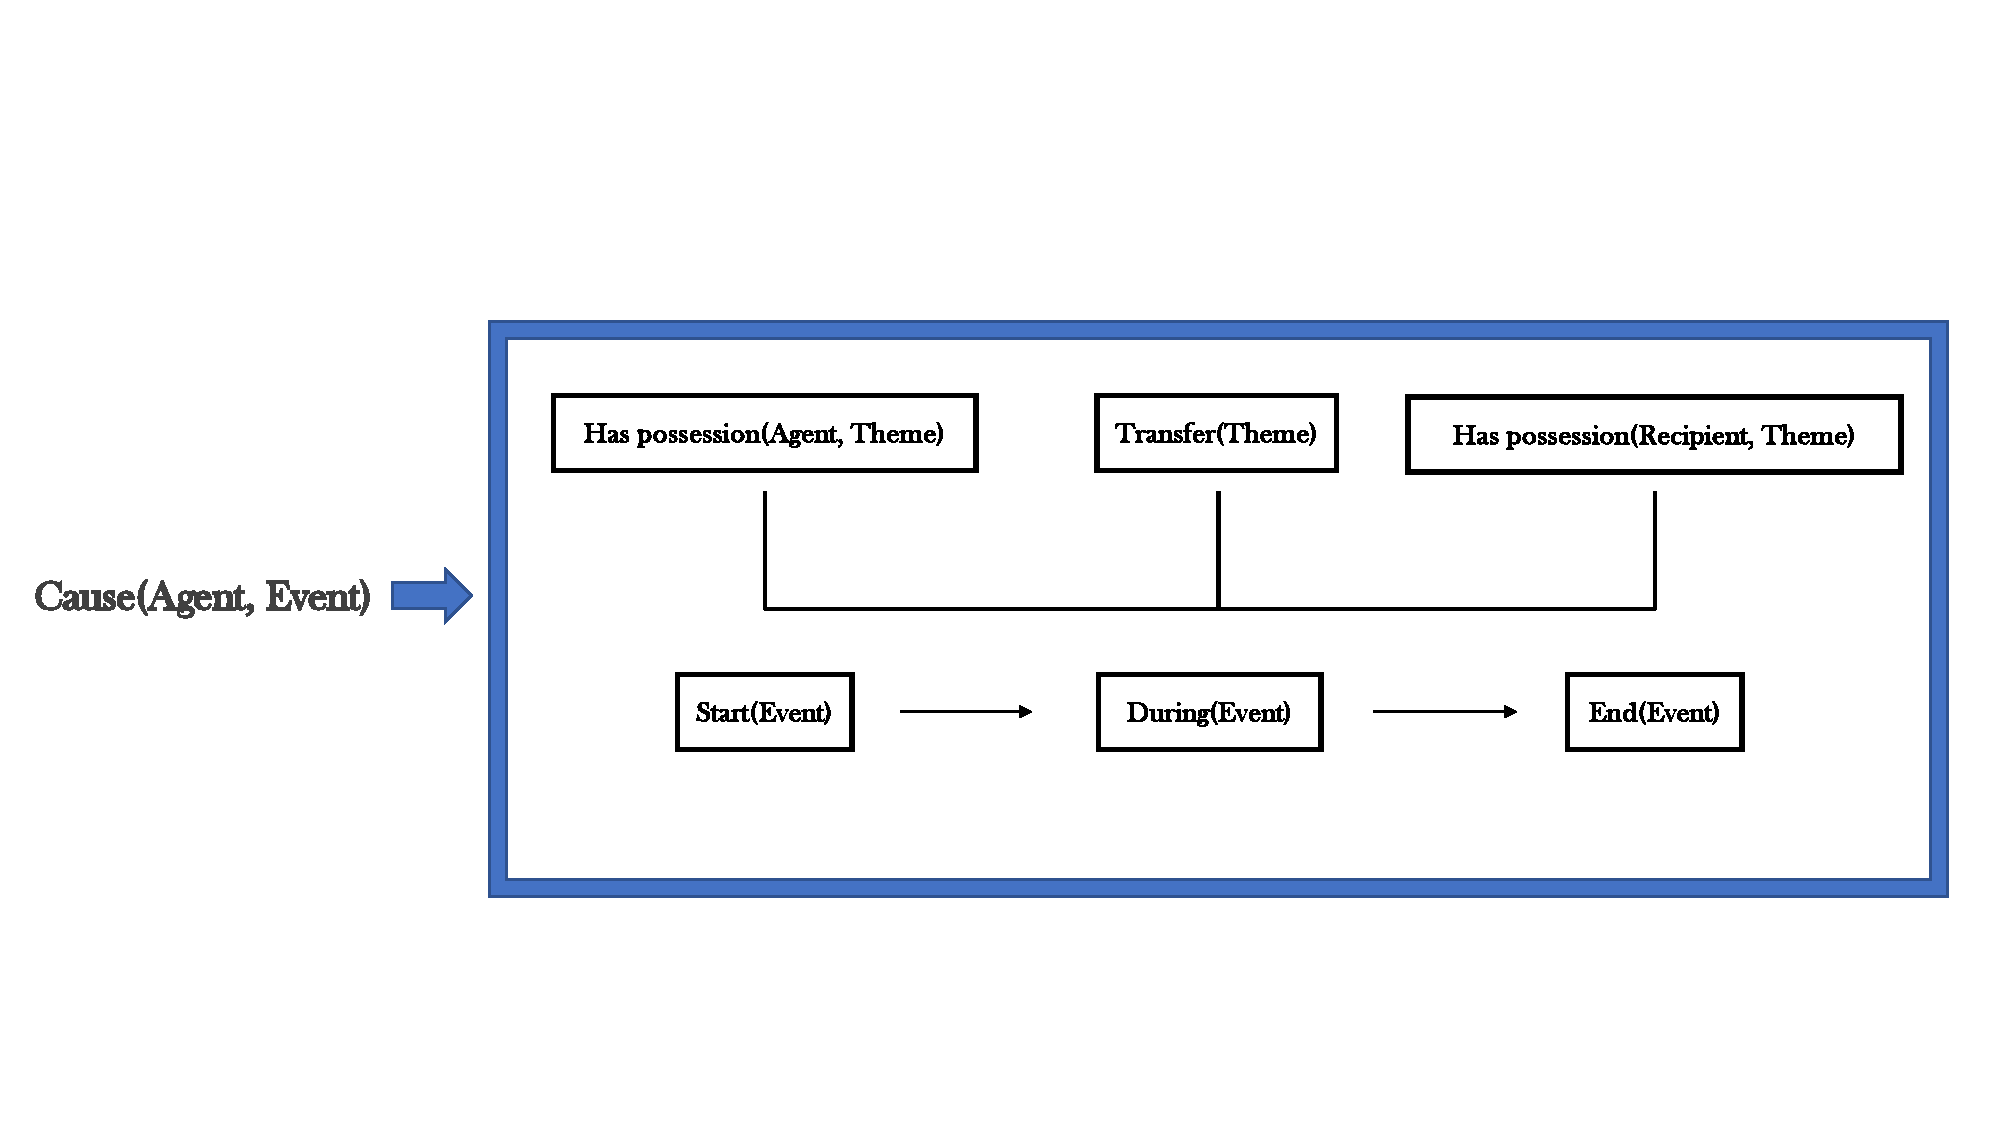
\includegraphics[width=1\textwidth, trim = {0cm 2cm 0cm 2cm},clip]{ch2/figs/semantics_give.pdf}
	\caption{prédicats sémantiques}
	\label{fig:Prédicat}
\end{figure}

\subsection{Brèves descriptions de dictionnaires concurrents utilisés en NLP}

\subsubsection{WordNet} : Wordnet est une base de données lexicale en ligne pour les verbes, noms, adjectifs et adverbes de la langue anglaise. Cette base de donnée est organisée en ensemble de synonymes, où chaque \emph{synset} contient des mots réferrant à un concept donné ainsi qu'une glose définition et une phrase exemple. L'aspect hiérarchique est construit via des liens d'hyperonymie et d'hyponomie entre les \emph{synsets}. Dans WordNet, les verbes sont classés parmi les classes suivantes s'il s'agit de verbes dénotant des actions ou des évènements (motion, perception, contact, communication, competition, change, cognition, consumption, creation, emotion, perception, possession, bodily care and functions, social behavior and interactions) et des verbes dénotant des états ( des types être :resemble, belong, suffice, des verbes contrôles (want, fail, prevent, succeed), et des verbes aspectuels (begin)) \citep{Fellbaum1998}

Les verbes sont groupés par ensemble de synonymes et non par classes verbales contrairement à VerbNet. Le concept de synonyme n'est pas vu dans son sens typique, il s'agit plus de : items lexicaux qu'on pourrait utiliser dans un même contexte sont vus comme des synonymes. À la base WordNet a été conçu pour agir comme réseau sémantique et contient ainsi peu d'information syntaxique. La ressource fournit des définitions, des exemples et des synsets, mais ne nous donne pas d'information sur la structure sémantique ou syntaxique des verbes, elle est sous-entendue, ce que fait que contrairement à VerbNet qui explicite en détail chaque patron de régime et structure syntaxique. les liens entre chaque items lexicaux sont de divers ordres : synonymes, antonymes, troponymes, entailment et causation.\citep{SchulerVerbnetBroadcoverageComprehensive2005}

"English verbs as a semantic net" \citep{Fellbaum1998} : Dans cet article, on exposer le liens sémantiques entre les verbes, ce que wordnet fait : il tisse un lien entre 2 verbes qui partagent des composantes sémantiques : ces liens sont de divers ordres et justifié par le concept d'entailment. Ainsi, on a les relations de hyponymie, hyperonymie, méronymie, troponoymie, etc.

D'ailleurs, VerbNet a décidé de faire un mapping de ses entrées lexicales aux entrées lexicales de WordNet pour complémenter la ressource. Chaque verbe dans VerbNet est mappé à WordNet si c'est possible et qu'il y existe un équivalent. On peut aussi confirmer le choix d'associer un mot à plusieurs classes verbales dans VerbNet. Ainsi, le verbe leave est associé à Escape, future having, keep, leave et fulfill car leave peut impliquer différentes composantes sémantiques en fonction des prédicats décrits dans ces classes. On retrouve l'équivalent dans les synset qui sont attribués à Leave (toutefois, WordNet attribue 14 différents sens à Leave) et VerbNet en attribue 5. Ainsi, lorsque c'est possible, les membres des classes se font assigné un WordNet ID avec. 

\subsubsection{FrameNet} : Le projet de Berkeley FrameNet contient de l'information sur les noms, adjectifs et verbes le tout basé sur un corpus annoté manuellement. Les sens des mots sont groupés dans des structures conceptuelles appelleés des Frames qui partageent des propriétés sémantiques similaires et qui sont des représentations de concepts cognitifs. La base de données FrameNet contient des descriptions des cadres sémantiques et des items lexicaux en association avec leur représentation sémantique et syntaxique en contexte (la représentation des valences). Le projet inclut aussi des phrases exemples pour les frames décrits. Les semantic frames sont définis comme des représentations schématiques de situations impliquant des participants , propositions et d'autres rôles conceptuels. Prenons le frame de JUDGEMENT qui possède les rôles : judge, evaluee, reason et le STATEMENT Frame avec des rôles comme SPEAKER, ADRESSEE et MESSAGE, tel que démontré en (2) et en (3). FrameNet utilise aussi le concept des rôles thématiques mais qu'ils appellent des Frames Elements qui agissent comme des étiquettes pour les divers arguments des verbes. Toutefois, dans FrameNet ces éléments sont spécifiques aux concepts du frame et non domain-independent, ainsi il en découlent de nombreux frame elements. Ça montre ici qu'on a plein de frame elements différents et ça n'apporte pas grand chose de les différencier, car en termes de fonction ils opèrent la même chose syntaxiquement.
suivi d'un exemple avec tableau pour montrer la différence entre un synset X et un frame X (prendre l'exemple de l'article de FrameNet)

FrameNet \citep{BakerBerkeleyFrameNetProject1998}: Les unités lexicales sont décrites en termes de frame semantics. Puis les unités lexicales ainsi que leurs frame semantics sont confirmées par des phrases exemples manuellement anotées sémantiquement provenant de corpus de la langue anglaise. Le but était encoder les connaissances sémantiques des unités lexicales dans une forme que les machines peuvent lire. Ils ont couvert les domaines sémantiques suivant : santé, chance, perception, communication, transaction, temps, espace, corps , motion, étapes de la vie, contexte sociaux, émotion et cognition. Ça nous donne une base de données lexicales. Qu'on décompose en 3 modules : 1 lexicon qui contient toutes les unités lexicales, une base de données de frames et les exemples annotées correspondant aux frames. La base de données de frames contient les descrptions des frames qui sont encodées en structures conceptuelles. Et les phrases exeples manuellement annotées sont des preuves empiriques que les frames ont lieu d'être. Les frames veulent décrire la structure argumentielle des unités lexicales. Ces arguments sont décrits par des étiquettes similaires aux rôles thématiques, mais beaucoup plus vastes car il y a différentes étiquettes en fonction du frame en question. On les appelle des frames elements et ceux-ci sont en lien avec le frame dont ils font partie. À noter qu'il y existe aussi une organisation hiérarchique où on a des sous-frames qui héritent de traits des frames parents. En frame semantics, un frame correspond à un scénario qui implique une intéraction et des participants (ceux-ci jouent un rôle dans l'intéraction)\citep{Shi:2005:PPT:2132047.2132058}

utilisation en NLP: On a combiné VN et FN pour en faire un semantic parser.\citep{Shi:2005:PPT:2132047.2132058}. Semantic parser : Au lieu de faire un parse tree syntaxique, ça fait un parse tree sémantique et ça nous recrée un arbre en tenant compte des participants et de leur relation avec le verbe et entre eux. 

mapping à VerbNet:\citep{Shi:2005:PPT:2132047.2132058} Le mapping s'est fait en deux étapes. d'abord, il fallait mapper les entrées lexicales de VN avec des frames appropriés de FN. Ensuite, il fallait mapper les rôles sémantiques de VN avec les frames elements de FN.

\subsubsection{XTAG} : Les chercheurs du projet XTAG ont construit une grammaire de la langue anglaise en se basant sur le formalisme de TAG (Tree Adjoining Grammar). Elle offre des descriptions riches des verbes en anglais. Chaque item lexical se fait assigner un ensemble d'arbres décrivant ses propriétés syntaxiques de base. Les arbres reflètent la structure prédicat-argument de ces items. Les arbres peuvent se combiner en deux opérations : subsitution et adjonction. En adjoignant de nouvelles branches ou en substituant des branches, la grammaire TAG permet de rendre compte des divers phénomènes linguistiques de la langue anglaise. La grammaire de XTAG inclut des descriptions syntaxiques pour 33 000 items lexicaux dont 9000 verbes et un éventail de 1300 arbres décrits et organisés en 70 famille d'arbres.
(parler du mapping)

a lexicalized tree adjoining grammar for English \citep{ResearchGroupLexicalizedTreeAdjoining2001}
Les arbres dans des familles d'arbres sont liés par le fait qu'ils représentent les mêmes type de cadres de sous-catégorisation. Ce qui distingue 2 arbres dans une même famille est des alternances syntaxiques. Les classes verbales sont organisées ainsi : Chaque verbe dans le lexicon syntaxique est associé à plusieurs familles d'arbres, où chaque famille regorge d'arbres individuels issues de différentes transformation syntaxiques mais ayant un cadre de sous-catégorisation les unissant. Ainsi, de cette manière un même verbe peut pointer vers différents arbres individuels, en passant par les familles d'arbres, et en étant associé à diverses familles d'arbres. Ainsi, ils n'ont pas à spécifier tous les arbres individuels qu'un verbe peut prendre, mais des familles d'arbres. Les familles d'arbres sont ainsi créées en prenant une forme canonique d'un cadre de sous-catégorisation et de lui faire toutes les transofmrations que permettent la langue anglaise, puis de générer les arbres en découlant avec les 2 opérations et storer le tout dans la base de données d'arbres de XTAG.

XTAG system \citep{DoranXTAGSystemWide1994}
Ce que fait XTAG, une phrase en input, puis on la fait passer par deux filtres : un analyseur morphologique et un POS tagger. Maintenant qu'on a des unités lexicales étiquettées et morphologiquement annotées. Ce filtrage augmente la rapidité du parsing. Puis le parser poursuit avec les unités qui lui sont fournis pour faire sa job de parser. Le parser consulte la base de données syntaxiques et la base de données d'arbres pour trouver l'arbre approprié pour chaque item lexical. Puis le parser combine les arbres élémentaires avec les 2 opérations adjonctions/substitution ce qui donne en output le parsing de la phrase donnée en input. Le travail similaire qui a été fait est la base de données d'arbres qui sont regroupés en famille d'arbres. La base de données syntaxiques pointe vers les arbres associées à chaque entrée lexicale, ou les familles d'arbres. On distingue arbre individuel (généralement non-verbaux) vs famille d'arbres (généralement des verbes) car les familles d'arbres représentent des cadres de sous-catégorisation. Les arbres dans une famille d'arbre 
sont liés entre eux par des transformation (changement de diathèse)

Assigning XTAG trees to VerbNet\citep{W04-3326}
Les auteurs de VerbNet ont ainsi voulu mapper leurs cadres syntaxiques aux arbres de XTAG.
Ça a permis d'étendre leur coverage à d'autres constructions syntaxiques. Comme XTAG a tenté de répertorier toutes les transformations possibles qu'une cadre de sous-catégorisation peut subir, il y avait bcp de matière. VerbNet couvre surtout la voix déclarative, tandis que XTAG explore toutes les transformations possibles. Mais ne fait pas de distinctions pour les différents sens des verbes et ne traite pas de sémantique. (juste dire qu'il y existe un mapping) et qu'ils sont allés étendre leur coverage un peu.


\subsubsection{Lexical conceptual structures}
La base de données de Dorr provient des théories de Jackendoff qui argumente en faveur d'une approche de décomposition sémantique pour la sémantique des verbes en termes de leur structure conceptuelle lexicale\citep{DorrUseLexicalSemantics1992}. Un LCS c'est un graphe, c'est une représentation sémantique et le lexique, les verbes sont encodés ainsi et dans la structure conceptuelle on voit la structure syntaxique qui découle des primitifs sémantiques. Une structure est composée de : représentation hiérarchique non linéraire, il y a une tête logique (la racine du graphe), un sujet logique (un seul) , des arguments logiques et des modificateurs logiques. L'élément principal d'un LCS sont des constituents conceptuels, les primitifs conceptuels et les champs sémantiques. Les constituents conceptuels appartiennent à un ensemble de catégories : chose, évènement, état, lieu, chemin, propriété, but, manière, montant, temps. Les champs sémantiques sont des traits comme : +temp, +loc, +poss qui agissent comme des restrictions sélectionnelles. Les primitifs conceptuels :ÊTRE, ALLER, RESTER , CAUSER, INCHOATIF, EXTENSION. Une décomposition sémantique des verbes en termes de structures lexicales conceptuelles explique leur propriété syntaxiques. Un peu comme Levin l'avait perçue, les propriétés sémantiques des verbes vont influencer leur comportements syntaxiques. Avec ce formalisme, on pense que les verbes avec des LCS similaires partagent aussi des comportement syntaxiques comme des alternances de diathèses. Ils utilisent aussi des rôles thématiques pour montrer la structure argumentale. La base de données de Dorr prend aussi la hiérarchie de Levin pour structure son information. Ainsi, les verbes sont classés en fontion des classes LCS. La base de donnée de Dorr LCS,inclue une grande quantité de verbes organisés en classes sémantiques dérivés des classifications de Levin.

Une structure LCS capture la sémantique d'une classe de verbe. Ainsi, tous les membres d'une classe partage la même structure sémantique, mais c'est le contenu sémantique qui diffère à l'intérieur de cette classe pour satisfaire les contraintes lexicales des verbes. \citep{TraumGenerationLexicalConceptual2000}. Un graphe LCS est une représentation sémantique où il y a des noeuds dont une racine. Chaque noeud a des spécifications avec des types d'information comme : type, primitif et champ. Type ; event, state, path, manner,etc. Puis après avoir spécifier le type, on spécifie le primitif sémantique du verbe (être, aller, rester,etc.)  et les champs sont des traits qui agissent comme des restrictions sur les noeuds.

Les auteurs de VerbNet trouvent qu'il y a un manque du côté des structures syntaxiques qui sont beaucoup trop simplifiées, et du fait que le lien entre la sémantique et la syntaxe n'est pas clair. Et une grande partie de ces données avaient été cherchées automatiquement menant à des incohérences, c'est pourquoi, après avoir fait une analyse des données ils n'ont pris que très peu d'information provenant de LCS.\citep{SchulerVerbnetBroadcoverageComprehensive2005}

Application en NLP : A été utilisé pour faire de la traduction automatique entre des langues différentes\citep{DorrUseLexicalSemantics1992}.  Pour le projet UNITRAN,espagnol, anglais et allemand. À l'aide de représentation basées sur la LCS , ils pouvaient fournir un input sémantique qui ensuite pouvait s'appliquer aux langues traitées et générer des traductions équivalentes entre les langues en utilisant leur lexicon et la théorie LCS. Une représentation sémantique qui pourra s'appliquer aux trois langues. Et les lexicons respectifs se chargent des spécificiéts de chaque langues.

\subsubsection{Comlex}
Base de données en anglais, développée à NYU. C'est une ressource syntaxique riche, mais qui n'est pas accessible au public. Chaque item lexical a des traits syntaxiques et  des compléments. Il existe 92 sous-catégorisation disponibles pour les verbes. Contient des descriptions syntaxiques pour 6000 verbes.  Selon les auteurs de VerbNet, il ne fait pas de distinction entre les différents sens d'un verbe (ce qui est problématique), et ne traite pas de sémantique explicitement. Mais il s'agit d'une base de données sur les constructions syntaxiques des unités lexicales qu'ils traitent.

Le but de Comlex était de \citep{Grishman:1994:CSB:991886.991931} créer un dictionnaire syntaxique sur les verbes de l'anglais à des fins computationelles. Ils ont opté pour un theory-neutral système. Surtout orienté subcategorization frame. Une entrée de dictionnaire contient :  la POS, les verbes qui prennent des compléments auront un trait sous-catégorisation. Il y aussi moyen de préciser des traits plus précis lorsqu'un verbe demande des particularités. Toutes les entrées sont faites manuellement car il ne pensait pas que des méthodes automatiques pouvait bien rendre compte des verbes moins fréquents, et ils voulaient que leurs entrées sois flawless.

\subsubsection{LexSchem}
A large subcategorization lexicon for french verbs \citep{MESSIANT08.142} L'auteur postule une automatisation de la tâche. La tâche étant la création d'un lexicon. L'information la plus utile qu'un lexicon peut offrir, sont les cadres de sous-catégorisation des verbes (la structure prédicat-argument). Les SCF capturent au niveau syntaxique les différentes combinaisons d'arguments qu'un prédicat peut prendre. Des lexicons de sous-catégorisation peuvent être très bénéfiques à des applications NLP. Peuvent être utilisés pour le parsing, la classification sémantique, extraction d'information et traduction automatique. L'acquisition automatique a fait ses preuves dans des applications réelles, bien que contrairement à l'approche manuelle, elle n'est pas aussi accurate et detailed. Ce qui est utile, ce sont les statistiques, la fréquence d'utilisation d'un SCF par rapport à un autre pour un verbe donné. Développé un système qui faisait une acquisition automatique des SCF en français à partir de corpus non-annoté. Les SCF acquis automatiquement sont incorporés dans lexSchem. D'abord, ils prennent des données brutes. Tag et lemmatise les mots , pour ensuite parser le tout , et commencer à en extraire les SCF. Les entrées lexicales sont composées essentiellement de : L'unité, ses cadres de sous-catégorisation et des phrases exemples tirées de corpus ainsi que la fréquence d'utilisation du SCF. (Acquis automatiquement, pourrait être intéressant pour le français à notre système et l'amener vers un GATM très riche syntaxiquement).

\subsubsection{A large SCF lexicon for NLP apps : Valex} \citep{Korhonenlargesubcategorizationlexicon2006}
Commence son article en justifiant pourquoi créer un lexicon verbal automatiquement est la meilleure manière de fonctionner de nos jours. Elle commence avec l'argument qu'il existe déjà des lexicons verbaux fait manuellement, mais que ceux-ci sont proies à faire des erreurs et que c'est coûteux en termes de temps à entretenir et à enrichir. Une information clé qu'on ne retrouve pas dans les dictionnaires manuellement encodés, ce sont les statstiques d'utilisation d'un SCF pour un prédicat donné. Comme beaucoup de systèmes fonctionnent avec des méthodes probabilistes, de telles informations sont cruciales à leur bon fonctionnement. Selon eux, ce genre d'information est quasi-impossible à encoder manuellement. C'est pourquoin elle postule l'acquisition des SCF automatique pour créer un dictionnaire, en extrayant les trucs via des textes non annotés. Les dictionnaires qui pratiquent cette méthode focusent que sur les verbes, ils rassemblent de l'information sur les cadres de sous-catégorisation. Mais ne différencie pas les sens des verbes, 80-85 \% de token recall. Ce ne sont pas des dictionnaires hautement précis : différencie pas les sens des verbes, pas de mapping entre la représentation syntaxique et la représentation sémantique, pas toujours les alternances de diathèses.

Voici comment le lexicon est créé : Ils ont utilisé le système d'acquisition de Briscoe et Caroll \citep{BriscoeSecondReleaseRASP2006} capable de catégoriser 163 cadres de sous-catégorisation et retournant la fréquence des SCF. Ce sytème utilise la méthode RASP. Donc des données brutes sont d'abord tokénisées, étiquettées, lématisées puis parsées utilisant RASP. Puis les SCF sont extraits des phrases parsées. Puis les patrons de régime sont classés dans l'une des 163 types de SCF. Ainsi, chaque entrée lexicale est en fait une combinaison verbe/SCF ce qui donne le lexicon de base. Puis, il est filtré car, puisque c'est une méthode automatique, le système trouve des SCF qui n'en sont peut-être pas, ou bien qui sont mal formés, etc. il faut donc les retirer du dictionnaire. Il y a aussi le problème, que certains SCF ne seront pas extraits puisqu'ils ne seront pas perçus comme étant des SCF selon le système. Ainsi, il faut pallier à ces problèmes et pour ce faire ils utilisent des méthodes statistiques pour améliorer le rappel/précsion. Et ils utilisent des dictionnaires construits manuellement pour trouver des SCF manquant. 

Une entrée lexicale dans le dictionnaire comprend entre autre : la combinaison d'un verbe et d'un SCF, la syntaxe des arguments, la fréquence d'utilisation du SCF, les POS des tokens.

\subsubsection{VDE-Valency dictionary of English}
Le VDE est un dictionnaire de patron de régime/valence/cadre de sous-catégorisation, etc.  Les dictionnaires de valence donne des informations sur les unités lexicales par rapport à la manière dont elles se combinent (le type d'argument que les verbes sélectionne, etc.). Ces ressources sont précieuses pour les applications NLP si on veut analyser la richesse d'une langue correctement. \citep{PROISL10.62}Le VDE contient la description de valence pour 511 verbes (et des noms et des ajdectifs). Chaque entrée démontre une valence possible pour un verbe accompagné d'un exemple provenant de Bank of English. À la base le projet n'était pas destiné à une application NLP, mais les auteurs se sont rendus compte qu'il y avait un marché-là, notamment du côté de LFG qui s'y prête bien pour des applications NLP. Ainsi est né Erlangen Valency Pattern Bank qui vise surtout les constructions syntaxiques possibles. Ainsi, le projet du Pattern Bank découle du VDE qui se prête bien à des applications NLP. Le pattern bank veut donner des outils pour la recherche en linguistique sur la valence. Ça liste les patrons de valence identifié pour les verbes par le VDE. Pour chaque patron de valence, une liste des unités lexicales pour le patron.  Les 511 verbes ont été choisi sur la base qu'ils sont fréquents dans la langue anglaise, démontre des propriétés complexes et sont utiles pour des apprenants de l'anglais. Les patrons de valence qu'on retrouve dans le VDE proviennent d'une étude de corpus fait sur le COBUILD. Les patrons sont décrits en termes de syntaxe de surface. Ne tient pas compte de description sémantique. 2 verbes peuvent pointer vers les mêmes patrons de valence s'ils ont la même structure. Dans le VDE, on donne l'information sur les participants, ce qui permet de distinguer 2 verbes différents qui partagent les mêmes patrons de valence, mais ils ne partageront pas toute la même information sémantique, c'est là qu'on précise les traits des participants. Mais, ces infos ne se retrouvent pas dans le Pattern Bank. Les patrons de valence sont identifiés par les compléments qui les remplisse. Ils distinguent les sens des lexèmes (accept au sens de approve vs integrate) et ainsi les différents patrons de valence incluent. De même que la différence des patrons entre voix passive et voix active. 

Donc, couvre peu de verbes, mais pourrait extraire ce qu'ils ont et le mapper à ce qu'on a déjà. On sait que c'est du travail qui a été fait manuellement, donc devrait pas avoir de truc de fou.

%Thomas Herbst and Peter Uhrig. 2009. Erlangen Valency Pattern Bank – a corpus-based research tool for work on valency and argument structure constructions. Website. http://www.patternbank.uni-erlangen.de

\subsubsection{Dicovalence}

Est un dictionnaire de valence pour la langue française. Le dictionnaire comprend les cadres syntaxiques de 3700 verbes. Une entrée lexicale dans ce dictionnaire est la combinaison d'un cadre valenciel et du verbe. Ainsi, puisque la plupart des verbes comptent plus d'un cadre valenciel, il y a plus de 8000 entrées lexicales dans ce dictionnaire. Les informations à l'intérieur des cadres valenciels sont présentés dans le cadre de l'approche pronominale en syntaxe (citation). Ce que plusieurs appellent des participants, des actants, des arguments, etc. sont ici appelés des paradigmes. A été créé dans une optique de TAL et d'enseignement de la langue. Ainsi une entrée est composée du cadre valenciel en termes de paradigme. Ce qui fait que le cadre valenciel de supprimer est composé de p0 p1, une sorte de description brève de la syntaxe de l'entrée. Dans ce jargon, p0 est l'équivalent du sujet et p1 de l'objet direct, puis p2 de l'objet indirect, et les autres p sont des obliques (quantité, temps, manière, locatif, délocatif,etc.). Contient aussi des phrases exemples, les traductions du verbe en anglais et en allemand, le frame en soi avec des restrictions sélectionnelles sur les paradigmes et d'autres informations grammaticales classiques : le type d'auxiliaire et les reformulations passives possibles.

\subsection {Utilisation de VerbNet dans des applications NLP}

VerbNet a été utilisé dans un nombre impressionnant de travaux de recherche. Ce qui en témoigne de son efficacité et de sa réputation. Voici notamment quelques projets de recherche où les chercheurs se sont servis de cette base de données lexicales pour effectuer leurs travaux.
Tâche : faire 3 lignes par article et décrire rapidement en quoi VerbNet a été utile pour ces travaux.

automatically building conceptual graphs using VerbNet and WordNet

Putting Pieces Together: Combining FrameNet, VerbNet and WordNet for Robust Semantic Parsing

Question Answering with Lexical Chains Propagating Verb Arguments
A question answering system based on VerbNet frames

a supervised algorithm for verb desambiguasation into VerbNet classes
semantic classifications for detection of verbs metaphor
VerbNet class assignment as a wsd task

multilingual NLG within abstractive generation.

\subsection{Pourquoi on n'a pas utilisé les rôles thématiques et les prédicats sémantiques}

Parler de ça dans la section python où on crée les patrons de régime, ça s'y prêtre plus.
p.210 dans le livre Melcuk
on pourrait garder les rôles pis les mettre dans MATE aussi

\subsection{Évaluation du système}
chapitre 5, p.75 C'est important de parler de l'évaluation du système car c'est celui que nous utiliserons, et nous voulons voir les problèmes qu'ils ont rencontré. Pour ensuite comparer avec l'utilisation que nous en aurons fait et à quel point les bons points selon eux ne sont peut-être pas les mêmes bons points que nous avons vu. Est-ce que VerbNet contient des coquilles car il a été créé par un processus automatique ? Voir la dissertation. (automatic techniques for extending coverage)

\subsection{Pourquoi avoir choisi VerbNet ?}

Expliquer pourquoi on a choisi VerbNet parmi tous les dictionnaires qui s'offraient à nous (en excluant ceux dans d'autres langues).



%%%%%%%%%%%%%%%%%%%%%%%%%%%%%%%%%%%%%%%%%%%%%
% ---------  P Y T H O N  ---------
%%%%%%%%%%%%%%%%%%%%%%%%%%%%%%%%%%%%%%%%%%%%

\section{Python}

À l'aide du module \emph{xml.etree.cElementTree} nous avons pu faire des opérations sur l'ensemble des données de VerbNet qui sont encodées dans des fichiers XML. Le module Etree nous permet de naviguer dans les fichiers XML de VerbNet puis de manipuler et d'extraire les données qui nous intéresse. Après avoir manipulé et extrait les données intéressantes, nous les avons compilées dans des dictionnaires. Ceux-ci seront utilisés par notre système MATE pour générer du texte automatiquement. Par la suite, nous avons aussi utilisé Python et le module Etree pour extraire les phrases exemples qui accompagent chaque patron de régime couvert par la ressource lexicale. Dans le but de créer des structures sémantiques qui nous serviront d'input pour générer en syntaxe de surface la phrase exemple et ainsi vérifier si MATE est capable de générer les phrases exemples.

Nous voulions donc créer des documents DICT qui seraient l'information lexicale de notre système de GAT. Il est d'abord important de dire dans les grandes lignes comment notre système MATE fonctionne. Ainsi, notre système prend en input une représentation sémantique d'un énoncé, puis fait appel à des dictionnaires et des règles de grammaire pour générer en output une représentation syntaxique de surface de l'énoncé. Les unités lexicales s'encodent d'une certaine manière dans MATE et nous voulions créer nos dictionnaires à l'image des contraintes données par le système MATE. Nous avons donc codé la manipualtion et l'extraction des données en fonction de la manière dont le lexique est encodé dans MATE.

\subsection{Création du dictionnaire de verbes: lexicon.dict}

La première étape de notre projet consistait à créer le dictionnaire verbal. Bien que le dictionnaire final comporte 6393 entrées lexicales verbales, cette partie de code nous permettait de créer la base de notre système. Il serait important de décrire dans les grandes lignes à quoi ressemble le dictionnaire pour mieux expliquer pourquoi nous l'avons extrait de cette manière. Ainsi MATE possède la caractéristique d'héritage des traits. Donc, en ce qui concerne les verbes, nous avons architecturé la chose de cette manière. Il existe une classe des verbes qui ont les traits suivants : une dpos=V et une spos=verb.

\begin{lstlisting}[language=XML]
verb {
  dpos = V
  spos = verb
}
\end{lstlisting}

Ensuite, les 278 classes verbales de VerbNet pointent vers la classe verb, donc les classes héritent de ces deux traits. Ce qui fait en sorte qu'on n'a pas a répété dans chaque entrée de classe verbale les traits dpos et spos. 

\begin{lstlisting}[language=XML]
"absorb-39.8": verb {
  gp = { id=NP_V_NP                        dia=12 } // Cotton absorbs water.
  gp = { id=NP_V_NP_PP_from_source         dia=123 } // Cattle take in nutrients from their feed.
}
\end{lstlisting}

Ensuite, chaque membre de chaque classe verbale pointe vers la classe ou la sous-classe qui le représente ce qui fait en sorte qu'il hérite de tous les traits de la classe(sous-classe) vers laquelle il pointe. Par exemple : absorb, ingest, take in vont tous trois hériter des traits de l'entrée "absorb-39.8" qui est la classe verbale. C'est de cette manière que notre dictionnaire passe de 278 entrées lexicales à 6393. Car, les verbes de la langue anglaise ont été classés dans des classes verbales et nous les intégront à notre dictionnaire en gardant la même architecture que VerbNet avait pensé (basé sur les travaux de Levin).

\begin{lstlisting}[language=XML]
absorb : "absorb-39.8"
take_in : "absorb-39.8"
ingest_1 : "absorb-39.8"
\end{lstlisting}

\subsubsection{Création du dictionnaire initial contenant les 278 classes verbales comme entrées lexicales}

\begin{lstlisting}[language=Python, caption = code pour lexicon.dict]
# BLOC 1
def supers(t, i):
    ID = t.get('ID')
    sc = {ID:i}
    subclasses = t.findall('SUBCLASSES/VNSUBCLASS')
    if len(subclasses) > 0:
        for sub in subclasses:
            sc = {**sc, **supers(sub, ID)}
    return sc
		
# BLOC 2
def treeframes(t):
    ID = t.get('ID')
    z = []
    for frame in t.findall('FRAMES/FRAME'):
        description = re.sub(r"\s*[\s\.\-\ +\\\/\(\)]\s*", '_', 
        frame.find('DESCRIPTION').get('primary'))
        if description in exclude:
            continue
        description = re.sub('PP', 'PP_{}', description)
        preps = [p.get('value') or 
                p.find('SELRESTRS/SELRESTR').get('type').upper() 
                for p in frame.findall('SYNTAX/PREP')+frame.findall('SYNTAX/LEX')]
        preps = [sorted(p.split()) for p in preps]     
        examples = [e.text for e in frame.findall('EXAMPLES/EXAMPLE')]
        if len(preps)==1:
            description = description.format('_'.join(preps[0]))
        elif len(preps)==2:
            description = description.format('_'.join(preps[0]),
                                             '_'.join(preps[1]))
        elif len(preps)==3:
            description = description.format('_'.join(preps[0]), 
                                             '_'.join(preps[1]), 
                                             '_'.join(preps[2]))
        z.append((description, examples))
        
    subclasses = t.findall('SUBCLASSES/VNSUBCLASS')
    subframes = [treeframes(subclass) for subclass in subclasses]
    subframes = sum(subframes, []) # flatten list of lists
    return [(ID, z)] + subframes
		
# BLOC 3
with open('lexicon.dict','w') as f:
    f.write('lexicon {\n')
    for file in [f for f in os.listdir('verbnet') if f[-4:] == '.xml']:
        root = ET.parse('verbnet/'+file).getroot()       
        d = dict(treeframes(root))
        sc = supers(root, 'verb')
        for c in d.keys():
            f.write('"'+c+'"')
            if sc[c] == 'verb':
                f.write(': ' +sc[c] + ' {')
            else :
                f.write(': ' +'"'+sc[c]+'"' + ' {')
            [f.write('\n  gp = { id=' + gp[0] + (max(len(gp[0]), 30)-len(gp[0]))
                     *' ' + ' dia=x } // ' + ' '.join(gp[1])) for gp in d[c]]
            f.write('\n}\n')
    f.write('\n}')
\end{lstlisting}

(Peut-être rajouter les numéros de lignes, ce sera utile pour faire référence à des lignes de code)
Ce premier script Python se découpe en trois blocs. Les deux premiers blocs sont des fonctions que nous définissons pour ensuite les utiliser dans le BLOC 3 qui nous permettra d'écrire le dictionnaire initial.  Ainsi, pour une meilleure compréhension du script complet, nous décrirons les blocs 1 et 2 pour expliquer ce que les fonctions font, ensuite nous décrirons le bloc 3 car l'usage des fonctions sera maintenant clair.

Commençons par la première fonction supers. La fonction prend 2 arguments : t et i. Si vous regardez le bloc 3, dans la section sc, on voit que supers prend les arguments (root, 'verb'). Ces deux arguments sont les suivants : root donne accès à l'arbre XML et 'verb' est fait pour que chaque classe verbale pointe vers la catégorie verbe. Pour en hériter les traits dpos=V et spos=verb.  On va chercher le trait ID dans l'un des deux arguments (l'argument arbre donc montré dans listing le trait ID dans le XML). Ensuite on crée un dictionnaire s'appelant sc dont la clé est le ID et la valeur est i. Puis on instancie une variable subclasses qui contient les racines de chaque sous-classes dans les documents XML (montrer avec listings à quoi ça ressemble dans le document XML). Puis ensuite, pour chaque élément dans sous-classe (si élément il y a) on lui passe la fonction supers et on va chercher son identifiant car en lui repassant la fonction, on retourne a sub.get('ID') donc on va chercher le ID qui se retrouve dans la partie sous-classe de l'arbre de la classe verbale et on met à jour le dictionnaire sc en y ajoutant les identifiants des sous-classes (les clés) qui pointeront vers l'identifiant de la classe qui le gouverne, car le deuxième argument de supers est une chaîne de caractère, dans ce cas, la chaîne ID qu'on avait pu chercher plus tôt dans la fonction. Cela est fait dans le but de construire: sous-classe : classe (donc la sous-classe hérite des traits de sa classe) grâce au mécanisme d'héritage de MATE, et tel que VerbNet le mentionne, chaque sous-classe hérite des traits donnés par la classe qui la domine. 

Maintenant, passons à la seconde fonction treeframe. Cette fonction prend un argument. On va aller chercher ID. Puis on initialise une liste z. Pour tous les frames qu'on retrouve dans l'arbre en question, on va chercher la description primaire du frame. On va ensuite se servir des expressions régulières pour uniformiser les descriptions à notre bon vouloir. Parallèlement, nous avons aussi créé une liste s'appelant exclude qui contient toutes les descriptions que nous voulons exclure de notre système et si une description dans un frame se retrouve aussi dans exclude, alors on n'y touche pas et elle ne sera pas modifiée ni ajoutée à la liste description. Ensuite, on modifie encore le nom des descriptions car nous ferons une opération par la suite. Donc, on modifie toutes les descriptions qui contiennent PP pour qu'elles ressemblent à 


%Nous avons donc utilisé VerbNet de mieux que nous le pouvions. Ainsi, les descriptions des FRAMES SYNTACTIC étaient "accurates" et allait nous donner les brèves descriptions des patrons de régime que nous ajouterons à notre lexiconCar, nous pensions au départ que nous pourrions tout prendre de verbnet pour créer notre lexicon.  Nous voulions chercher les descriptions des patrons de régime ainsi que l'information sous SYNTAX sous FRAME pour ainsi créer les patrons de régime en soi en les traduisant dans notre langage (TST). Toutefois, leur manière d'encore les patrons de régime ne correpond pas à la notre sur beaucoup trop d'aspect. Nous le verrons plus tard, il y a de la redondance à certains moments et notre théorie rend mieux compte des patrons de régime. Mais pour l'instant, ce qui est important de noter c'est que nous notons les patrons de régime en attribuant des actants I et des noms de relation pour signifier que est le rôle de cet actant lors du passage de la sémantique à la syntaxe. VerbNet ne fait pas cela de la même manière que nous. Ils ont aussi un volet sémantique, mais qui ne se branche pas à notre modèle théorique. Nous voulions donc nous inspirer quand même de leur méthode pour nos patrons de régime, mais le fait qu'ils utilisent les rôles thématiques nous posait problème. Il était difficile d'associer un rôle thématique à un actant syntaxique (bien que nous ayons tenté [montrer le graphique de F.L]). Donc, nous en sommes venus à la conclusion qu'il nous faudrait créer les patrons de régime en Python pour ensuite les exporter dans un format adéquat pour MATE. Pour ce faire, nous devions utilisé les descriptions des patrons de régime qui se retrouve dans \emph{ VerbNet} et à partir de la description, créer une fonction qui nous permettrait de générer rapidement des patrons de régime adéquat pour MATE en ayant simplement à remplir les trous. 

%Pour extraire les descriptions des patrons de régime nous avons utilisé deux fonctions. D'abord la fonction \emph{treeframe} qui s'occupe de récupérer la description de chaque frame syntaxique à travers tout VN. Nous passons à travers tous les frames existant dans les XML de VN. Autant dans les classes que les sous-classes. Toutefois, cette fonction ne fait pas que récupérer la description du syntactic frame de VN et nous la recrache tel quel. Nous faisons quelques opérations sur les descriptions que nous extrayons. Notamment, nous remplaçons tout espace,tiret, point,barre oblique, paranthèses qui pourraient se trouver dans les descriptions par des {\_} à l'aide d'expressions régulières. Puis, nous retirons certaines descriptions de gp à cause de leur caractèrere problématique à encoder(pour des raisons théoriques, logiques -- à expliquer ailleurs).Puis une fois qu'un clean up a été fait des descriptions et que nous avons uniquement celles que nous voulions, nous procédons à une seconde étape de raffinement des descriptions. Nous utiliserons une seconde fois une expression régulière pour trouver tous les occurrences de PP car nous ajouterons les prépositions impliquées dans les PP comme tel. Pour ce faire, nous faisons un search de tous les prépositions existant dans les patrons de régime de verbnet(et non dans la description, c'est là que les patrons de régime de VN nous ont été utiles) et nous mettons les prépositions que nous soutirons des gp directement dans le nom de la description des gp à la suite du mot PP à chaque fois qu'on retrouve le mot PP dans une description. On obtient ainsi les descriptions nettoyées de celle qu'on ne veut pas, avec uniquement des underscore pour séparer les syntagmes puis les prépositions (lorsqu'il y a lieu) dans les noms des descriptions de gp.

%Puis, une fois que nous faisions ces opérations sur les classes de VerbNet, nous avons scripté une méthode pour que la fonction s'applique aussi aux sous-classes.

%Par la suite, nous avons créé une fonction \emph{super} afin que la création du lexicon s'agence bien avec la manière que MATE fonctionne. Cette fonction nous permet d'utiliser le mécanisme d'héritage qui existe dans MATE. Ainsi, on peut renvoyer une sous-classe à la classe(ou sous-classe) qui la domine. De plus, cette fonction limite le nombre de descriptions de gp. VerbNet a aussi ce mécanisme d'intégrer autrement. Ainsi, si une classe X a 10 descriptions et qu'une sous-classe Y en a 5, mais que les 10 descriptions de la classe s'appliquent aussi à la sous-classe, on n'aura pas 15 descriptions mais juste 5 dans le sous-classe, car le mécanisme d'héritage s'occupe de faire ça. On a aussi programmé la création den notre lexicon pour que si il n'y a pas de sous-classes, que la classe hérite de la classe verb afin d'avoir les attributs de base de cette classe (la dpos, la spos, voir MATE). De cette manière, tous les classes héritent de la classe verb si on remonte aux classes mères, ainsi, on n'a pas besoin de préciser à chaque fois la dpos/spos.

%Puis finalement, nous  utilisons la fonction write qui écrit le tout dans un fichier .dict. Nous loopons à travers tous les fichiers compris dans le dossier VN. Puis nous allons chercher les keys et values du dictionnaire créé à l'aide de la fonction treeframe et du dictionnaire super.(À revoir)

%Nous avons aussi pris la peine d'extraire les exemples pour chaque description car il s'agit d'une information utile pour voir dans quel contexte s'utilise ce patron de régime. Et c'est une information pertinente à avoir dans un dictionnaire, donc nous l'ajouterons à notre lexicon pour notre système de GAT. Pour ce faire, nos opérons de la même manière que pour les descriptions de gp dans le sens où nous faisons l'extractiond exemples en passant par les feuilles XML et le module d'extraction xml.etree. Pour chaque frame, nous passons la fonction à l'entièreté de VN et nous nous arrêtons à la balise EXAMPLES puis à tout texte se trouvant dans cette balise. Nous avons voulu extirper les exemples alongside des descriptions car c'est de l'information pertinente à avoir dans un dictionnaire.

\subsubsection{Extraction des 6393 membres des classes verbales pour enrichir le dictionnaire lexicon.dict}

\begin{lstlisting}[language=Python, caption = code pour ajouter des lexèmes à lexicon.dict]
def treemember(t):
    ID = t.get('ID')
    members = [m.get('name') for m in t.findall('MEMBERS/MEMBER')]
    subclasses = t.findall('SUBCLASSES/VNSUBCLASS')
    submembers = []
    if len(subclasses) > 0:
        for sub in subclasses:
            submembers = submembers + treemember(sub)
    return [(ID, members )] + submembers

files = [f for f in os.listdir('verbnet') if f[-4:] == '.xml']

members = dict(sum([treemember(ET.parse('verbnet/'+file).getroot()) for file in files], [])) # ici on a classe : [membre,...]
values = sum(list(members.values()), []) # ici c'est uniquement les membres, sans infos sur leur classe
dups = {m:[ID for ID in members.keys() if m in members[ID]] for m in values if values.count(m)>1}
unique_member = {m:ID for ID in members.keys() for m in values if m in members[ID] and values.count(m)==1}
lexemes = {d[0]+'_'+str(n+1):d[1][n] for d in dups.items() for n in range(len(d[1]))}

# Ici, je fusionne les dictionnaires ensemble
unified_dict = {**unique_member, **lexemes}

with open('members.dict','w') as f:
    f.write('members {\n')
    for key in sorted(unified_dict.keys()):
        f.write(key)
        f.write(' : '),
        f.write('"'+str(unified_dict[key])+'"')
        f.write('\n')
    f.write('\n}\n')

\end{lstlisting}

\subsection{Création du gpcon}

\begin{lstlisting}[language=Python, caption = code pour gpcon.dict]
def roman(n):
    return ['I', 'II', 'III', 'IV', 'V', 'VI'][n-1]
		
def gp(name, real_actant):
    s = name + ' {\n'
    i=0
    for actant in real_actant:
        i = i+1
        if type(actant) == list:
            for y in actant:
                s = s + "   " + roman(i) + "={" + y + "}\n"
        else:
            s = s + "   " + roman(i) + "={" + actant + "}\n"
    s = s + '}\n'
    return s


#SUBJECTIVE
subj = 'rel=subjective dpos=N'

#DIRECT OBJECTIVE
dir_N = 'rel=dir_objective dpos=N'
dir_V_ING = 'rel=dir_objective dpos=V finiteness=GER'
dir_V_INF = 'rel=dir_objective dpos=V finiteness=INF'

#INDIRECT OBJECTIVE
to_N = 'rel=indir_objective dpos=N prep=to'
indir_N = 'rel = indir_objective dpos = N'

#OBLIQUE
on_V = 'rel=oblique dpos=V prep=on'
to_obl_N = 'rel=oblique dpos=N prep=to' 
for_obl_N = 'rel=oblique dpos=N prep=for'
as_N =  'rel=oblique dpos=N prep=as'
against_N = 'rel=oblique dpos=N prep=against'
at_N = 'rel=oblique dpos=N prep=at'

# LOC

locab = 'rel=oblique dpos=N prep=locab'
locad = 'rel=oblique dpos=N prep=locad'
locin = 'rel=oblique dpos=N prep=locin'

descriptions = {
'NP_agent_V' : [subj],
'NP_agent_V_NP' : [subj, dir_N],
'NP_asset_V_NP_PP_from_out_of' : [subj, dir_N, [from_N, out_of_N]],
'NP_attribute_V' : [subj],
'NP_attribute_V_NP_extent' : [subj, dir_N],
'NP_attribute_V_PP_by_extent' : [subj,by_N],
'NP_cause_V_NP' : [subj, dir_N ],
'NP_instrument_V_NP' : [subj, dir_N],
'NP_location_V' : [subj],
'NP_location_V_NP_theme' : [subj,dir_N],
'NP_location_V_PP_with_agent' : [subj, with_N],
'NP_location_V_PP_with_theme' : [subj, with_N],
'NP_material_V_NP' : [subj,dir_N],
'NP_material_V_PP_into_product' : [subj, into_N],

# CREATION DU GPCON
with open('gpcon.dict','w') as f:
    f.write('gpcon {\n')
    for d in descriptions.keys():
        f.write(gp(d, descriptions[d]))
    f.write('}')

\end{lstlisting}

Rajouter aussi en lstlistings les résultats qui sont des documents .dict (à la fin de l'explication)

Soit le mentionner ici, ou ailleurs, mais il a fallu faire un dictionnaire de patron de régime. D'abord, parce qu'on s'est rendu compte que du à toute l'information qu'on allait chercher et la différence dans le type d'information, on a jugé bon de créer un second dictionnaire qui ne contiendrait que les gps, autrement dit un gpcon. Celui l'information sur les patrons de régime (les actants syntaxiques). Il existe x nombre de gps répertoriés. Nous les avons trouvé en faisant un ensemble à partir de tous les descriptions que nous avons obtenus avec le script précédent. Une fois que nous avons l'ensemble des gps différents. Il nous fallait les créer, car tel que mentionné, nous ne pouvions pas extraire les gps de VerbNet dû à une différence trop grande (cadre théorique et application). Notre système de GAT fonctionne avec la théorie Sens-Texte et nous pensons que c'est la théorie qui s'y prête le plus pour faire ce type d'opérations et qui tient le mieux compte de la manière dont le langage fonctionne. Ainsi, nous avons créer le gpcon à partir de Python car un bon nombre d'opérations peuvent être automatisés (éviter les fautes, et c'est plus transparent). Pour la création du gpcon, notre dictionnaire en Python ressemblait à ça. Nos keys() étaient la description du gp et les valeurs étaient les actants syntaxiques impliqués dans ce gp (avec de l'information sur les actants syntaxiques nécessitant une préposition à réaliser). Selon l'ordre dans lequel figure nos objets dans la liste qui est ce qu'on retrouve dans values(), notre fonction va assigner le bon actant syntaxique(I, II, III, etc.) ainsi, cette partie est automatisée grâce à cette fonction. Après, pour l'objet "subj" on va lui assigner une string 'rel=subjective dpos=N' ce qui est encodé dans une autre cellule. Ainsi à chaque fois qu'un gp a  un subj, on n'a pas à écrire ce que subj contient. Alors pour l'objet subj, on aura I et 'rel=subjective dpos=N'. C'est l'union de la fonction gp et de la fonction roman qui nous permettent d'assigner les bons actants syntaxiques aux objets dans la liste qui représente les values dans mon dictionnaire de gpcon.

\subsection{Scripts pour faire les tests}

\subsubsection{Extraction des exemples}

\begin{lstlisting}[language=Python, caption = code pour créer phrases.txt]
def treeframes(t):
    z = []
    for frame in t.findall('FRAMES/FRAME'):
        description = re.sub(r"\s*[\s\.\-\ +\\\/\(\)]\s*", '_', frame.find('DESCRIPTION').get('primary'))
        if description in exclude:
            continue    
        examples = [e.text for e in frame.findall('EXAMPLES/EXAMPLE')]
        z =  z + examples 
    subclasses = t.findall('SUBCLASSES/VNSUBCLASS')
    subframes = [treeframes(subclass) for subclass in subclasses]
    subframes = sum(subframes, []) # flatten list of lists
    return z + subframes

liste=[]
with open('phrases.txt','w') as f:
    for file in [f for f in os.listdir('verbnet') if f[-4:] == '.xml']:
        root = ET.parse('verbnet/'+file).getroot()       
        d = (treeframes(root))
        final_liste = liste + d
        [f.write(x+'\n') for x in final_liste]

\end{lstlisting}

\subsubsection{Création des structures qui serviront de tests}

Dans la figure ci-bas, on explique comment on a créer les documents .str qui serviront d'input à notre système MATE qui prend ce genre de document en entrée.

\begin{lstlisting}[language=Python, caption = code pour créer des structures .str]
phrases = open('phrases.txt','r')

with open('structures.str','w') as f:
    for(i,p) in enumerate(phrases):
        with open('s'+str(i)+'.str','w') as g:
            structure = 'structure Sem S'+str(i)+'{\n S {text="'+p.strip()+'"\n\n main-> \n }\n}'
            f.write(structure)
            g.write(structure)
\end{lstlisting}

\chapter{Génération automatique de texte}

Pour cette partie, prendre l'article en 8 pages de François, et observer comment il décrit le déroulement de MATE. Reprendre l'idée, mais approfondir chaque point

Ce sera une section du mémoire sur le mécanisme dsynt=X

\section{Mécanisme dsynt=created->constrained->OK pour générer un énoncé simple (sujet, verbe, objet)}

\subsection{Application de la règle root{\_}standard}
Cette règle crée un noeud qui sera la racine de l'arbre syntaxique. Ce noeud se fait imposer des contraintes. Notamment, on demande à ce que ce soit un lexème appartenant à la partie du discours : verbe et que sa finitude soit de type: fini. On impose à ce noeud le trait dsynt=constrained pour que ça s'harmonise avec le règle lex{\_}standard, mais c'est à revoir.

\subsection{application de la règle lex{\_}standard pour lexicaliser le verbe principal}
On assigne un lexème à un noeud  créé en syntaxe profonde. Dans le contexte actuel, on l'utilise pour sélectionner l'unité lexicale qui matche les contraintes énoncées sur le noeud vide créé par la règle root{\_}standard. Ce lexème provient du lexicon. Lorsque la règle s'applique et qu'elle consomme le noeud en y mettant la bonne lexicalisation (qui respecte les contraintes sur le noeud), on ajoute un trait dsynt=OK pour signifier que le sémantème a été réalisé en syntaxe profonde et qu'on ne fasse plus d'opérations sur ce noeud.

\subsection{Application de la règle actant{\_}gp{\_}selection}
Cette règle s'applique lorsque nous avons un prédicat.
On crée une variable[ ?GP] qui nous fournit un chemin vers l'information encodée sous l'attribut \emph{ gp} d'un lexème [?X]. Puis , on extirpe les traits \emph{ id} et \emph{dia} pour chaque attribut\emph{ gp} de notre [?X]. Une fois qu'on a récupéré ces informations, on les appose au lexème en question car on se servira de ces informations pour l'application de règles subséquentes. Le trait \emph{ id} représente la description du patron de régime (chaque description se retrouve dans notre gpcon qui est un dictionnaire de\emph{ gp}) et le trait dia nous renseigne sur la diathèse de ce patron de régime, c'est-à-dire combien d'actants sont en jeu, et dans quel ordre sont-ils placés ? Il est essentiel qu'un lexème verbal aille chercher ces traits car il en a besoin pour appliquer les règles actancielles qui en découlent. Il faut que le système sache quel patron de régime utilisé pour un prédicat donné, et dans quel ordre les actants seront réalisés en syntaxe.

\subsection{application des règles actancielles}
Une fois qu'un gp est sélectionné, on appliquera la règle actancielle qui lui correspond. Nos règles actancielles ressemblent à : actant{\_}gp{\_}ijk. Les règles prennent en input les arcs sémantiques liant les actants à leur prédicat. Ces règles génèrent des noeuds vides auxquels on appose un trait dsynt=created pour signifier qu'on vient de créer des noeuds vides (on dit qu'ils sont vides car ils n'ont pas encore été consommés par une unité lexicale) en syntaxe profonde. On obtient ainsi des arcs syntaxiques au bout desquels se trouve un noeud vide. Ces règles se font imposer des conditions bien strictes. Il faut d'abord que le prédicat qui les gouverne soit lexicalisé. Ce qui se traduisait par l'ajout d'un trait dsynt=OK au lexème lexicalisé (avec la règle lex{\_}tandard). La règle actant{\_}gp{\_}selection nous permettait de soutirer les traits  \emph{ id} et \emph{dia} et c'est ici que le trait dia entre en jeu. On s'en sert pour illustrer la diathèse du verbe. [à revoir]

\subsection{application de la règle constraints{\_}gp}
Cette règle applique des contraintes à des noeuds nouvellement créés (autrement dit, des noeuds qui ont le trait dsynt=created). C'est à partir de cette règle que le mécanisme de \emph{dsynt=created-> constrained->OK} prend vie. Il s'agit d'une étape intermédiaire entre la création du noeud avec les règles actancielles et la lexicalisation qui consommera le noeud en octroyant un lexème suivant un trait dsynt=OK (signifiant que la réalisation en syntaxe profonde est terminée). Ainsi, la règle procède de cette manière. On prend un X (un prédicat) qui lie un Y (un actant) puis ce dernier se fait imposer des contraintes. On cherche à lui imposer ces contraintes car on souhaite qu'il respecte le patron de régime de X. Ainsi, s'il ne convient pas comme actant syntaxique, il ne pourra pas passer à la lexicalisation. Car on souhaite une correspondance entre les traits naturels contenus dans le dictionnaire pour le sémantème en question. Si ses traits ne convienne pas aux contraintes imposées au noeud, provenant du patron de régime de X, alors l'arbre sera incomplet. Lorsqu'on met les contraintes sur le noeud, on lui met aussi le trait dsynt=constrained pour montrer qu'il a été contraint et donc qu'il remplit les critères pour passer à la lexicalisation.

\subsection{application des règles de lexicalisation}

Il y a différentes règles de lexicalisation afin de donner un peu de latitude au système. Ainsi, si quelques informations sont manquantes dans le lexicon ou le semanticon, nous voulons que le système arrive quand même à effectuer une génération de texte. C'est pourquoi il existe la règle standard qui fonctionne lorsque nous avons accès à tous les éléments nécessaires. Les régles de types \emph{guess} opèrent lorsqu'il nous manque certaines infos. 

\subsubsection{lex{\_}standard}

Nous avons vu cette règle un peu plus haut, car il fallait l'appliquer dès le début pour lexicaliser le noyau principal afin de chercher le bon lexème qui pouvait remplir cette fonction. Une fois que nous l'avons lexicalisé, nous avons pu aller chercher les informations sur la nature de son gp etc. Nous sommes maintenant rendus au moment où il existe des arcs syntaxiques au bout desquels nous avons des noeuds contraints par des traits comme : la dpos, la finitude, la définitude, etc. Nous allons donc lexicaliser ces noeuds afin de poursuivre la construction de l'arbre, du haut vers le bas. En gros, comment ça fonctionne. On cherche la lexicalisation d'un sémantème donné dans le semanticon, en allant chercher le trait \emph{lex} du sémantème. Puis, on colle cette lexicalisation a un noeud déjà existant. Ce noeud existe déjà car il a soit été créé par root{\_}standard ou par une des règles actancielles. On va octroyer au noeud 3 traits : un trait dlex, un trait dpos, et finalement un trait dsynt. Le trait dlex est la lexicalisation profonde, celle qu'on retrouve dans le lexicon, le trait dpos est la partie du discours profonde qui doit correspondre à la dpos demandée par constraints{\_}gp. Et finalement, un trait dsynt=OK qui s'ajoute à la lexicalisation du sémantème pour signifier au système que le noeud a été consommé et qu'il a été réalisé en syntaxe profonde. Donc, qu'on ne fasse plus d'opération sur ce noeud. Finalement, on peut uniquement faire des opérations sur des noeuds qui ont let trait dsynt=constrained afin de lexicaliser seulement les noeuds qui se sont fait attribués des contraintes. Ainsi, s'ils respectent les contraintes, ils pourront être lexicalisé, sinon, l'arbre sera incomplet et la génération échouera.

\subsection{Avantages d'utiliser ces mécanismes}

"Dsynt=OK" indique que le noeud a été consommé. Autrement dit, il existe maintenant une unité lexicale réalisé en syntaxe profonde, là où il y avait un noeud vide.
"Dsynt=constrained" indique qu'un noeud vide s'est fait imposé des contraintes. Ces contraintes peuvent être de plusieurs ordres. Notamment, on impose une dpos, une finitude, un mood, etc. Il s'agit du passsage intermédiaire entre la création d'un noeud et sa lexicalisation. On veut s'assurer qu'il respecte certaines contraintes pour ne pas lexicaliser n'importe quoi lors de la génération de notre arbre syntaxique.
Finalement, le trait dsynt=created 

\section{Énumérations}

Voici une énumération avec numérotation :
\begin{enumerate}
	\item item 1;
	\item item 2;
	\item item 3.
\end{enumerate}
Maintenant, une énumération sans numérotation avec des marqueurs différents :
\begin{itemize}
	\item Marqueur par défaut;
	\item[$\bullet$] \verb|$\bullet$|;
	\item[$\star$] \verb|$\star$|.
\end{itemize}


\section{Équations mathématiques}

Une équation :
\begin{equation*}
	\otimes^n\,\mathbb{C}^2 \cong \bigoplus_{m=-n/2}^{n/2} W_m.
\end{equation*}

Une autre équation, cette fois-ci numérotée :
\begin{equation}
	\label{eq:eulerlagrange}
	\frac{\partial\mathcal{L}}{\partial\phi^a}-\partial_\mu\frac{\partial\mathcal{L}}{\partial(\partial_\mu\phi^a)}=0,\qquad\mu=0,1,2,3.
\end{equation}
Les équations \eqref{eq:eulerlagrange} précédentes sont appelées \emph{équations d'Euler-Lagrange} ou encore \emph{équations du mouvement}. Dans les calculs suivants,
\begin{align*}
	\delta S	& = \int_\Omega\mathrm{d}^dx\,\mathcal{L}\bigl(\phi'^a(x),\partial_\mu\phi'^a(x)\bigr)-\int_\Omega\mathrm{d}^dx\,\mathcal{L}\bigl(\phi^a(x),\partial_\mu\phi^a(x)\bigr)																												\\
				& = \int_\Omega\mathrm{d}^dx\,\left[\delta\phi^a\frac{\partial\mathcal{L}}{\partial\phi^a}+\partial_\mu\delta\phi^a\frac{\partial\mathcal{L}}{\partial(\partial_\mu\phi^a)}\right]																									\\
				& = \int_\Omega\mathrm{d}^dx\,\left[(\delta\phi^a\frac{\partial\mathcal{L}}{\partial\phi^a}+\partial_\mu\left(\delta\phi^a\frac{\partial\mathcal{L}}{\partial(\partial_\mu\phi^a)}\right)-\delta\phi^a\partial_\mu\frac{\partial\mathcal{L}}{\partial(\partial_\mu\phi^a)}\right]	\\
				& = 0,
\end{align*}
aucune ligne n'est numérotée. Alors que dans ce qui suit, la derni\`ere ligne l'est :
\begin{align}
	\delta S	& = \int_{\Omega'}\mathrm{d}^dx'\,\mathcal{L}\bigl(\phi'^a(x'),\partial'_\mu\phi'^a(x')\bigr)-\int_\Omega\mathrm{d}^dx\,\mathcal{L}\bigl(\phi^a(x),\partial_\mu\phi^a(x)\bigr)																															\notag\\
				& = \int_\Omega\mathrm{d}^dx\,\left[\bar{\delta}\phi^a\frac{\partial\mathcal{L}}{\partial\phi^a}+\partial_\mu\bar{\delta}\phi^a\frac{\partial\mathcal{L}}{\partial(\partial_\mu\phi^a)}\right]+\int_{\partial\Omega}\mathrm{d}\sigma_\mu\,\mathcal{L}\bigl(\phi^a,\partial_\mu\phi^a\bigr)\delta x^\mu	\notag\\
				& = \int_\Omega\mathrm{d}^dx\,\partial_\mu\mathcal{J}^\mu(x).	\label{eq:variationaction}
\end{align}


\section{Définitions, théor\`emes et preuves}

Voici une définition.
\begin{deff}[La définition]
	La définition.
\end{deff}
Voici un théor\`eme.
\begin{theo}[Titre]
	Ceci est vrai !
\end{theo}
\begin{proof}
	Voici la preuve.
\end{proof}
\begin{demo}
	Voici la preuve en gras.
\end{demo}


\section{Construction d'un tableau}

\begin{table}[htb]
	\centering
	\caption{Un tableau simple dans le second chapitre.}
	\label{tab:simple2}
	\begin{tabular}{|c||l|c|r|p{0.4\textwidth}|}
		\hline			&			&			&			&																															\\
		\textbf{Option}	& g			& c			& d			& \verb|p{0.4\textwidth}|																									\\[3mm]
		\hline\hline	&			&			&			&																															\\
		\textbf{Effet}	& À gauche	& Au centre	& À droite	& Le texte de cette colonne est justifié et la largeur de la colonne est fixée \`a 40\,\% de la zone de texte (hors tableau).	\\[3mm]
		\hline 
	\end{tabular}
\end{table}
Le tableau \ref{tab:simple2} n'est pas tr\`es garni.

\section{Référence \`a une entrée bibliographique}

Les documents par \citet{Lamport1986,GMS1994} ainsi que \citet{Spivak1990} 
sont des références en mati\`ere de \LaTeX. Le manuel par 
\citet{GMS1994} est probablement le plus populaire du lot.

L'article de \citet{Martin1992} est, manifestement, tr\`es riche en rebondissements.

Les entrées du fichier \verb|.bib| qui ne sont pas référencées 
dans le texte ne sont pas ajoutées \`a la bibliographie : un avantage 
de plus en faveur de Bib\TeX.

Dans ce paragraphe, on teste une cette référence \citet{hastie2005}.

\section{Insertion de figures}

% Voici deux types d'insertion de figures.

\begin{figure}[t]
	\centering
	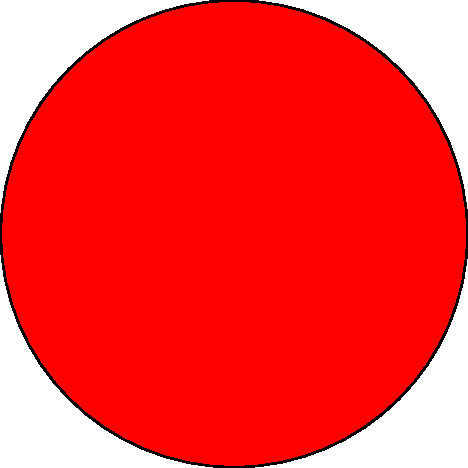
\includegraphics[width=0.2\textwidth]{ch3/figs/cercle.pdf}
	\caption{Un cercle.}
	\label{fig:Cercle}
\end{figure}

La figure \ref{fig:Cercle} est un \emph{cercle}.
\begin{figure}[t]
	\centering
	\subfigure[Un triangle.]{\label{fig:Triangle}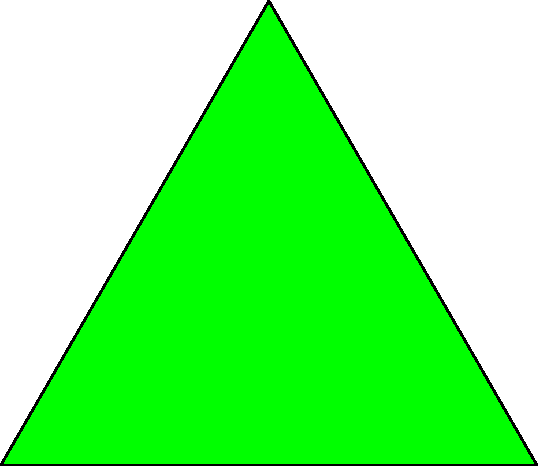
\includegraphics[width=0.2\textwidth]{ch3/figs/triangle.pdf}}\hspace{2cm}
	\subfigure[Un carré.]{\label{fig:Carre}
\includegraphics[width=0.2\textwidth]{ch3/figs/carre.pdf}}
	\caption{\label{fig:TriCar}Un carré et un triangle.}
\end{figure}
À la figure \ref{fig:TriCar}, le triangle \subref{fig:Triangle} et le carré \subref{fig:Carre} ont été placés côtes-\`a-côtes grâce \`a la commande \verb|\subfigure|. 





% Annexes
% Enlever le commentaire de \appendix pour faire vos annexes.
% Les annexes sont ensuites faites comme un chapitre normal : \chapter{nom_de_l'annexe}.
\appendix

%%%%%%%%%%%%%%%%%%%%%%%%%%%%%%%%%%%%%
%%   BIBLIOGRAPHIE                  %
%%%%%%%%%%%%%%%%%%%%%%%%%%%%%%%%%%%%%
  % Enlever les commentaires de la prochaine commande si vous préférez que le
  % chapitre s'appelle « Références » plutôt que « Bibliographie » (au choix selon le contexte).
%\let\bibname=\refname   

%% Lorsque vous serez prêt à faire afficher votre bibliographie
%% et vos références, enlevez les commandaires des commandes suivantes
%% et donnez le nom de votre fichier .bib à la commande \bibliography{..}
%% (consultez l'exemple au besoin).  Vous pouvez utiliser le style de votre
%% choix.  Le fichier francaissc.bst est inclus avec le gabarit.  Vous pouvez
%% utiliser ce style avec  \bibliographystyle{francaissc}
% 
\bibliographystyle{biblio/francaissc}		    % Le style de la bibliographie. Notons que les extensions ne sont pas données pour ces deux fichiers.
\bibliography{biblio/references}		    % La base de données contenant des entrées bibliographiques. Seules celles référencées dans le texte seront ajoutées \`a la bibliographie.

%!TEX root = ../memoire.tex

\chapter{Corpus d'évaluation}

Inputs et outputs de GenDR à partir des phrases tirées de VerbNet

\iffalse 
\begin{longtable}{@{}rp{10cm}@{}}
\caption{Phrases tirées de VerbNet pour l'évaluation}\\
\toprule
\textbf{Num} & \textbf{Phrase} \\
\midrule
\endfirsthead
\multicolumn{2}{c}%
{\tablename\ \thetable\ -- \textit{Suite}} \\
\toprule
\textbf{Num} & \textbf{Phrase} \\
\midrule
\endhead
\bottomrule \multicolumn{2}{r}{\textit{Suite à la page suivante}} \\
\endfoot
\bottomrule
\endlastfoot

17	&	I loved writing \\
27	&	They allow smoking \\
36	&	Plays and ballets alternate \\
77	&	I begged her to do it \\
111	&	The dragon breathed fire on Mary \\
142	&	Oils's price increased ten percent \\
177	&	The doctor cured Pat of pneumonia \\
198	&	She classified the works as `dangerous' \\
206	&	Cora coiled the rope around the post \\
213	&	The prime minister complained to the former president about U.S. interference in his country's affairs \\
222	&	The Milky Way comprises more than 100 billion planets \\
227	&	The children hid from Sally \\
244	&	They considered him professor \\
250	&	I spent the time on worries \\
264	&	Some of the members may donate privately \\
267	&	He converted to believing in Buddha \\
330	&	This flyer and that flyer differ \\
384	&	He entered the room \\
399	&	The bells traded places \\
426	&	We focused on it \\
428	&	We brooded about it \\
452	&	Carmen bought a dress for \$50 \\
476	&	The teacher gathered the kids \\
503	&	Smith was inscribing \\
540	&	We abandoned the area \\
554	&	Sasha dawdled in the museum \\
581	&	I anguished over Aslan's pain \\
583	&	Dina masqueraded as a lawyer \\
604	&	Herman added a computer to the network \\
618	&	I neglected to do the job \\
630	&	She laughed in embarrassment \\
667	&	Lydia pocketed the change in her left pocket \\
686	&	Donna grilled me steaks \\
688	&	The dealer valued the book \\
746	&	Tom jumped the horse over the fence \\
750	&	The horse jumped the stream \\
777	&	TransCanada is shifting its HQ to Calgary from Toronto \\
789	&	The crew spotted the island \\
836	&	The thief stole the paint for Mary \\
843	&	I ended the party with a speech \\
845	&	Winnie the Pooh subjugated the unfortunate Pixies \\
851	&	The streets gushed with water \\
862	&	The sailor drowned \\
868	&	Bees are swarming in the garden \\
873	&	Paula swatted the fly with a cloth \\
894	&	Ellen told Helen a story \\
900	&	Steve tossed the ball from the corner to the garden \\
955	&	Linda winked her eye \\
968	&	Barry Cryer erased the writing \\
974	&	He backed out of going on the trip \\

\end{longtable}
\fi

\begin{tabbing}
(17)\quad\= \emph{I loved writing.} \\
\> \begin{minipage}{16cm}
\raisebox{-0.5\height}{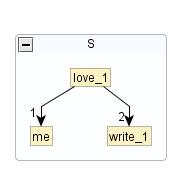
\includegraphics[scale=0.45]{{annexes/figs/test-eval-17.sem}.jpg}}
\raisebox{-0.5\height}{~$\Rightarrow$~}
\raisebox{-0.5\height}{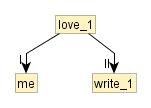
\includegraphics[scale=0.45]{{annexes/figs/test-eval-17.dsynt}.jpg}}
\raisebox{-0.5\height}{~$\Rightarrow$~}
\raisebox{-0.5\height}{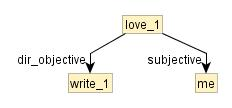
\includegraphics[scale=0.45]{{annexes/figs/test-eval-17.ssynt}.jpg}}
\end{minipage}
\end{tabbing}

\begin{tabbing}
(27)\quad\= \emph{They allow smoking.} \\
\> \begin{minipage}{16cm}
\raisebox{-0.5\height}{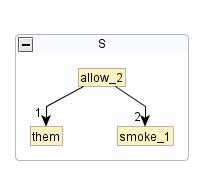
\includegraphics[scale=0.45]{{annexes/figs/test-eval-27.sem}.jpg}}
\raisebox{-0.5\height}{~$\Rightarrow$~}
\raisebox{-0.5\height}{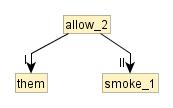
\includegraphics[scale=0.45]{{annexes/figs/test-eval-27.dsynt}.jpg}}
\raisebox{-0.5\height}{~$\Rightarrow$~}
\raisebox{-0.5\height}{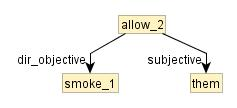
\includegraphics[scale=0.45]{{annexes/figs/test-eval-27.ssynt}.jpg}}
\end{minipage}
\end{tabbing}

\begin{tabbing}
(36)\quad\= \emph{Plays and ballets alternate.} \\
\> \begin{minipage}{16cm}
\raisebox{-0.5\height}{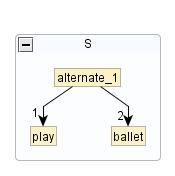
\includegraphics[scale=0.45]{{annexes/figs/test-eval-36.sem}.jpg}}
\raisebox{-0.5\height}{~$\Rightarrow$~}
\raisebox{-0.5\height}{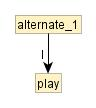
\includegraphics[scale=0.45]{{annexes/figs/test-eval-36.dsynt}.jpg}}
\raisebox{-0.5\height}{~$\Rightarrow$~}
\raisebox{-0.5\height}{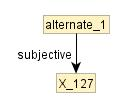
\includegraphics[scale=0.45]{{annexes/figs/test-eval-36.ssynt}.jpg}}
\end{minipage}
\end{tabbing}

\begin{tabbing}
(77)\quad\= \emph{I begged her to do it.} \\
\> \begin{minipage}{16cm}
\raisebox{-0.5\height}{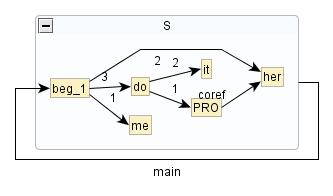
\includegraphics[scale=0.45]{{annexes/figs/test-eval-77.sem}.jpg}}
\raisebox{-0.5\height}{~$\Rightarrow$~}
\raisebox{-0.5\height}{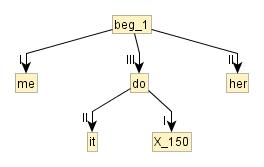
\includegraphics[scale=0.45]{{annexes/figs/test-eval-77.dsynt}.jpg}}
\\
\raisebox{-0.5\height}{~$\Rightarrow$~}
\raisebox{-0.5\height}{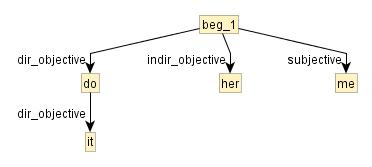
\includegraphics[scale=0.45]{{annexes/figs/test-eval-77.ssynt}.jpg}}
\end{minipage}
\end{tabbing}

\begin{tabbing}
(111)\quad\= \emph{The dragon breathed fire on Mary.} \\
\> \begin{minipage}{16cm}
\raisebox{-0.5\height}{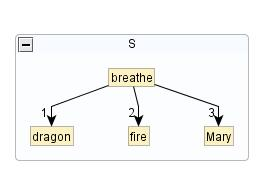
\includegraphics[scale=0.45]{{annexes/figs/test-eval-111.sem}.jpg}}
\raisebox{-0.5\height}{~$\Rightarrow$~}
\raisebox{-0.5\height}{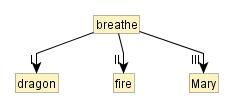
\includegraphics[scale=0.45]{{annexes/figs/test-eval-111.dsynt}.jpg}}
\raisebox{-0.5\height}{~$\Rightarrow$~}
\raisebox{-0.5\height}{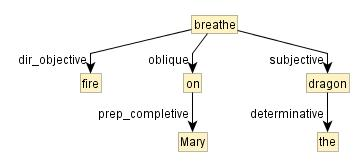
\includegraphics[scale=0.45]{{annexes/figs/test-eval-111.ssynt}.jpg}}
\end{minipage}
\end{tabbing}

\begin{tabbing}
(142)\quad\= \emph{Oils’s price increased ten percent.} \\
\> \begin{minipage}{16cm}
\raisebox{-0.5\height}{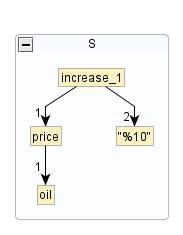
\includegraphics[scale=0.45]{{annexes/figs/test-eval-142.sem}.jpg}}
\raisebox{-0.5\height}{~$\Rightarrow$~}
\raisebox{-0.5\height}{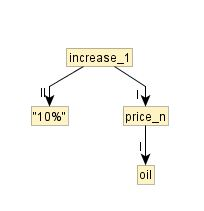
\includegraphics[scale=0.45]{{annexes/figs/test-eval-142.dsynt}.jpg}}
\raisebox{-0.5\height}{~$\Rightarrow$~}
\raisebox{-0.5\height}{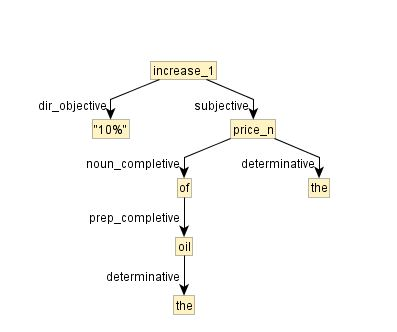
\includegraphics[scale=0.45]{{annexes/figs/test-eval-142.ssynt}.jpg}}
\end{minipage}
\end{tabbing}

\begin{tabbing}
(177)\quad\= \emph{The doctor cured Pat of pneumonia.} \\
\> \begin{minipage}{16cm}
\raisebox{-0.5\height}{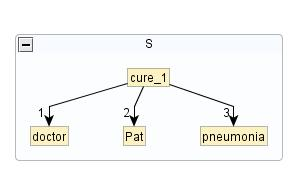
\includegraphics[scale=0.45]{{annexes/figs/test-eval-177.sem}.jpg}}
\raisebox{-0.5\height}{~$\Rightarrow$~}
\raisebox{-0.5\height}{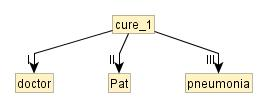
\includegraphics[scale=0.45]{{annexes/figs/test-eval-177.dsynt}.jpg}}
\raisebox{-0.5\height}{~$\Rightarrow$~}
\raisebox{-0.5\height}{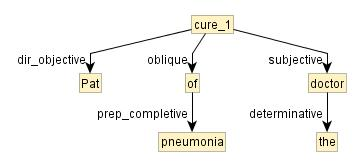
\includegraphics[scale=0.45]{{annexes/figs/test-eval-177.ssynt}.jpg}}
\end{minipage}
\end{tabbing}

\begin{tabbing}
(198)\quad\= \emph{She classified the works as 'dangerous'.} \\
\> \begin{minipage}{16cm}
\raisebox{-0.5\height}{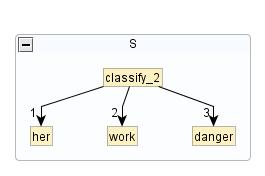
\includegraphics[scale=0.45]{{annexes/figs/test-eval-198.sem}.jpg}}
\raisebox{-0.5\height}{~$\Rightarrow$~}
\raisebox{-0.5\height}{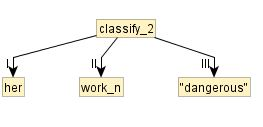
\includegraphics[scale=0.45]{{annexes/figs/test-eval-198.dsynt}.jpg}}
\raisebox{-0.5\height}{~$\Rightarrow$~}
\raisebox{-0.5\height}{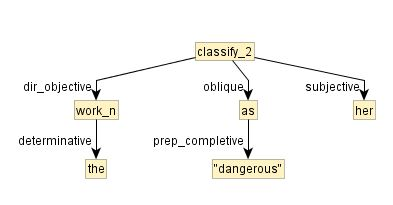
\includegraphics[scale=0.45]{{annexes/figs/test-eval-198.ssynt}.jpg}}
\end{minipage}
\end{tabbing}

\begin{tabbing}
(206)\quad\= \emph{Cora coiled the rope around the post.} \\
\> \begin{minipage}{16cm}
\raisebox{-0.5\height}{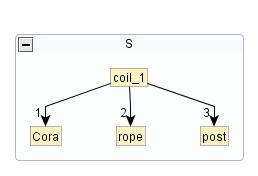
\includegraphics[scale=0.45]{{annexes/figs/test-eval-206.sem}.jpg}}
\raisebox{-0.5\height}{~$\Rightarrow$~}
\raisebox{-0.5\height}{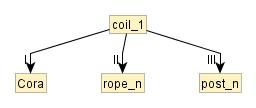
\includegraphics[scale=0.45]{{annexes/figs/test-eval-206.dsynt}.jpg}}
\raisebox{-0.5\height}{~$\Rightarrow$~}
\raisebox{-0.5\height}{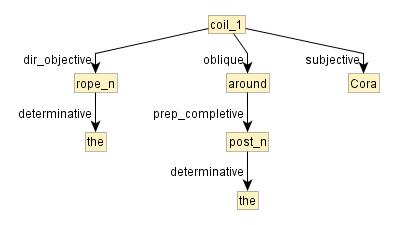
\includegraphics[scale=0.45]{{annexes/figs/test-eval-206.ssynt}.jpg}}
\end{minipage}
\end{tabbing}


\begin{tabbing}
(213)\quad\= \emph{The prime minister complained to the former president about U.S. interference} \\
          \> \emph{in his country’s affairs.} \\
\> \begin{minipage}{16cm}
\raisebox{-0.5\height}{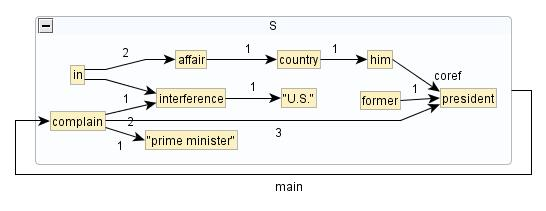
\includegraphics[scale=0.45]{{annexes/figs/test-eval-213.sem}.jpg}}
\raisebox{-0.5\height}{~$\Rightarrow$~}
\raisebox{-0.5\height}{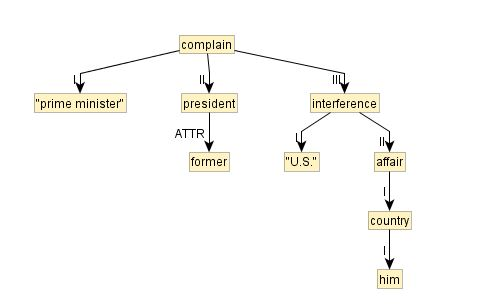
\includegraphics[scale=0.45]{{annexes/figs/test-eval-213.dsynt}.jpg}}
\raisebox{-0.5\height}{~$\Rightarrow$~}
\raisebox{-0.5\height}{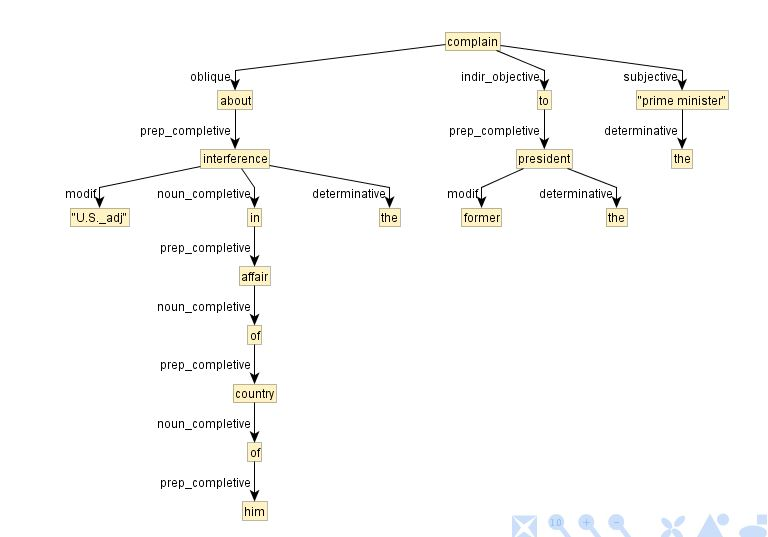
\includegraphics[scale=0.45]{{annexes/figs/test-eval-213.ssynt}.jpg}}
\end{minipage}
\end{tabbing}


\begin{tabbing}
(222)\quad\= \emph{The Milky Way comprises more than 100 billion planets.} \\
\> \begin{minipage}{16cm}
\raisebox{-0.5\height}{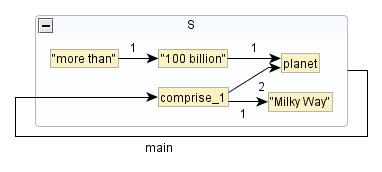
\includegraphics[scale=0.45]{{annexes/figs/test-eval-222.sem}.jpg}}
\raisebox{-0.5\height}{~$\Rightarrow$~}
\raisebox{-0.5\height}{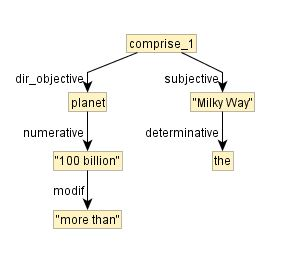
\includegraphics[scale=0.45]{{annexes/figs/test-eval-222.dsynt}.jpg}}
\raisebox{-0.5\height}{~$\Rightarrow$~}
\raisebox{-0.5\height}{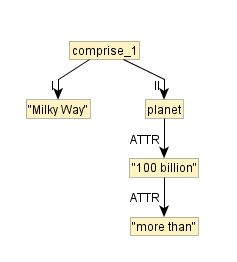
\includegraphics[scale=0.45]{{annexes/figs/test-eval-222.ssynt}.jpg}}
\end{minipage}
\end{tabbing}

\begin{tabbing}
(227)\quad\= \emph{The children hid from Sally.} \\
\> \begin{minipage}{16cm}
\raisebox{-0.5\height}{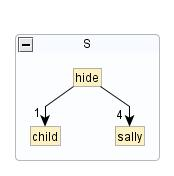
\includegraphics[scale=0.45]{{annexes/figs/test-eval-227.sem}.jpg}}
\raisebox{-0.5\height}{~$\Rightarrow$~}
\raisebox{-0.5\height}{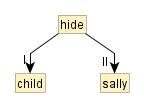
\includegraphics[scale=0.45]{{annexes/figs/test-eval-227.dsynt}.jpg}}
\raisebox{-0.5\height}{~$\Rightarrow$~}
\raisebox{-0.5\height}{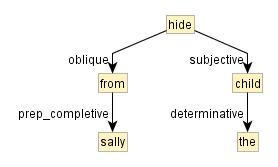
\includegraphics[scale=0.45]{{annexes/figs/test-eval-227.ssynt}.jpg}}
\end{minipage}
\end{tabbing}

\begin{tabbing}
(244)\quad\= \emph{They considered him professor.} \\
\> \begin{minipage}{16cm}
\raisebox{-0.5\height}{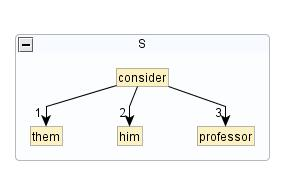
\includegraphics[scale=0.45]{{annexes/figs/test-eval-244.sem}.jpg}}
\raisebox{-0.5\height}{~$\Rightarrow$~}
\raisebox{-0.5\height}{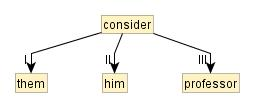
\includegraphics[scale=0.45]{{annexes/figs/test-eval-244.dsynt}.jpg}}
\raisebox{-0.5\height}{~$\Rightarrow$~}
\raisebox{-0.5\height}{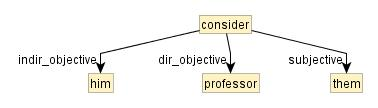
\includegraphics[scale=0.45]{{annexes/figs/test-eval-244.ssynt}.jpg}}
\end{minipage}
\end{tabbing}

\begin{tabbing}
(250)\quad\= \emph{I spent the time on worries.} \\
\> \begin{minipage}{16cm}
\raisebox{-0.5\height}{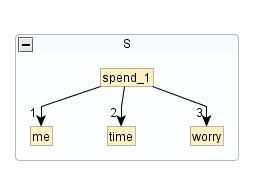
\includegraphics[scale=0.45]{{annexes/figs/test-eval-250.sem}.jpg}}
\raisebox{-0.5\height}{~$\Rightarrow$~}
\raisebox{-0.5\height}{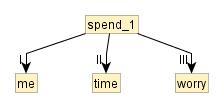
\includegraphics[scale=0.45]{{annexes/figs/test-eval-250.dsynt}.jpg}}
\raisebox{-0.5\height}{~$\Rightarrow$~}
\raisebox{-0.5\height}{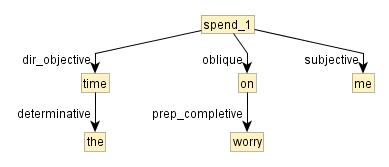
\includegraphics[scale=0.45]{{annexes/figs/test-eval-250.ssynt}.jpg}}
\end{minipage}
\end{tabbing}

\begin{tabbing}
(264)\quad\= \emph{Some of the members may donate privately.} \\
\> \begin{minipage}{16cm}
\raisebox{-0.5\height}{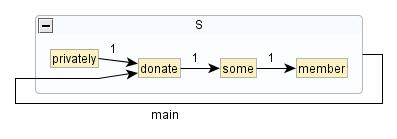
\includegraphics[scale=0.45]{{annexes/figs/test-eval-264.sem}.jpg}}
\raisebox{-0.5\height}{~$\Rightarrow$~}
\raisebox{-0.5\height}{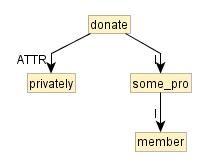
\includegraphics[scale=0.45]{{annexes/figs/test-eval-264.dsynt}.jpg}}
\raisebox{-0.5\height}{~$\Rightarrow$~}
\raisebox{-0.5\height}{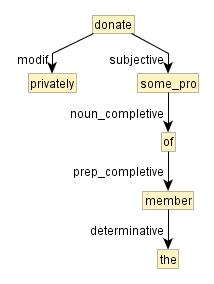
\includegraphics[scale=0.45]{{annexes/figs/test-eval-264.ssynt}.jpg}}
\end{minipage}
\end{tabbing}

\begin{tabbing}
(267)\quad\= \emph{He converted to believing in Buddha.} \\
\> \begin{minipage}{16cm}
\raisebox{-0.5\height}{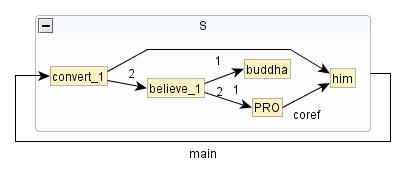
\includegraphics[scale=0.45]{{annexes/figs/test-eval-267.sem}.jpg}}
\raisebox{-0.5\height}{~$\Rightarrow$~}
\raisebox{-0.5\height}{\includegraphics[scale=0.45]{{annexes/figs/test-eval-267.dsynt}.jpg}}
\raisebox{-0.5\height}{~$\Rightarrow$~}
\raisebox{-0.5\height}{\includegraphics[scale=0.45]{{annexes/figs/test-eval-267.ssynt}.jpg}}
\end{minipage}
\\
\> \draft{Bla bla le noeud X...}
\end{tabbing}



\begin{tabbing}
(330)\quad\= \emph{This flyer and that flyer differ.} \\
\> \begin{minipage}{16cm}
\raisebox{-0.5\height}{\includegraphics[scale=0.45]{{annexes/figs/test-eval-330.sem}.jpg}}
\raisebox{-0.5\height}{~$\Rightarrow$~}
%\raisebox{-0.5\height}{\includegraphics[scale=0.45]{{annexes/figs/test-eval-330.dsynt}.jpg}}
\raisebox{-0.5\height}{~$\Rightarrow$~}
%\raisebox{-0.5\height}{\includegraphics[scale=0.45]{{annexes/figs/test-eval-330.ssynt}.jpg}}
\end{minipage}
\end{tabbing}

\begin{tabbing}
(384)\quad\= \emph{He entered the room.} \\
\> \begin{minipage}{16cm}
\raisebox{-0.5\height}{\includegraphics[scale=0.45]{{annexes/figs/test-eval-384.sem}.jpg}}
\raisebox{-0.5\height}{~$\Rightarrow$~}
\raisebox{-0.5\height}{\includegraphics[scale=0.45]{{annexes/figs/test-eval-384.dsynt}.jpg}}
\raisebox{-0.5\height}{~$\Rightarrow$~}
\raisebox{-0.5\height}{\includegraphics[scale=0.45]{{annexes/figs/test-eval-384.ssynt}.jpg}}
\end{minipage}
\end{tabbing}

\begin{tabbing}
(399)\quad\= \emph{The bells traded places.} \\
\> \begin{minipage}{16cm}
\raisebox{-0.5\height}{\includegraphics[scale=0.45]{{annexes/figs/test-eval-399.sem}.jpg}}
\raisebox{-0.5\height}{~$\Rightarrow$~}
\raisebox{-0.5\height}{\includegraphics[scale=0.45]{{annexes/figs/test-eval-399.dsynt}.jpg}}
\raisebox{-0.5\height}{~$\Rightarrow$~}
\raisebox{-0.5\height}{\includegraphics[scale=0.45]{{annexes/figs/test-eval-399.ssynt}.jpg}}
\end{minipage}
\end{tabbing}


\begin{tabbing}
(426)\quad\= \emph{We focused on it.} \\
\> \begin{minipage}{16cm}
\raisebox{-0.5\height}{\includegraphics[scale=0.45]{{annexes/figs/test-eval-426.sem}.jpg}}
\raisebox{-0.5\height}{~$\Rightarrow$~}
\raisebox{-0.5\height}{\includegraphics[scale=0.45]{{annexes/figs/test-eval-426.dsynt}.jpg}}
\raisebox{-0.5\height}{~$\Rightarrow$~}
\raisebox{-0.5\height}{\includegraphics[scale=0.45]{{annexes/figs/test-eval-426.ssynt}.jpg}}
\end{minipage}
\end{tabbing}

\begin{tabbing}
(428)\quad\= \emph{We brooded about it.} \\
\> \begin{minipage}{16cm}
\raisebox{-0.5\height}{\includegraphics[scale=0.45]{{annexes/figs/test-eval-428.sem}.jpg}}
\raisebox{-0.5\height}{~$\Rightarrow$~}
\raisebox{-0.5\height}{\includegraphics[scale=0.45]{{annexes/figs/test-eval-428.dsynt}.jpg}}
\raisebox{-0.5\height}{~$\Rightarrow$~}
\raisebox{-0.5\height}{\includegraphics[scale=0.45]{{annexes/figs/test-eval-428.ssynt}.jpg}}
\end{minipage}
\end{tabbing}

\begin{tabbing}
(452)\quad\= \emph{Carmen bought a dress for 50\$.} \\
\> \begin{minipage}{16cm}
\raisebox{-0.5\height}{\includegraphics[scale=0.45]{{annexes/figs/test-eval-452.sem}.jpg}}
\raisebox{-0.5\height}{~$\Rightarrow$~}
\raisebox{-0.5\height}{\includegraphics[scale=0.45]{{annexes/figs/test-eval-452.dsynt}.jpg}}
\raisebox{-0.5\height}{~$\Rightarrow$~}
\raisebox{-0.5\height}{\includegraphics[scale=0.45]{{annexes/figs/test-eval-452.ssynt}.jpg}}
\end{minipage}
\end{tabbing}

\begin{tabbing}
(476)\quad\= \emph{The teacher gathered the kids.} \\
\> \begin{minipage}{16cm}
\raisebox{-0.5\height}{\includegraphics[scale=0.45]{{annexes/figs/test-eval-476.sem}.jpg}}
\raisebox{-0.5\height}{~$\Rightarrow$~}
\raisebox{-0.5\height}{\includegraphics[scale=0.45]{{annexes/figs/test-eval-476.dsynt}.jpg}}
\raisebox{-0.5\height}{~$\Rightarrow$~}
\raisebox{-0.5\height}{\includegraphics[scale=0.45]{{annexes/figs/test-eval-476.ssynt}.jpg}}
\end{minipage}
\end{tabbing}

\begin{tabbing}
(503)\quad\= \emph{Smith was inscribing.} \\
\> \begin{minipage}{16cm}
\raisebox{-0.5\height}{\includegraphics[scale=0.45]{{annexes/figs/test-eval-503.sem}.jpg}}
\raisebox{-0.5\height}{~$\Rightarrow$~}
\raisebox{-0.5\height}{\includegraphics[scale=0.45]{{annexes/figs/test-eval-503.dsynt}.jpg}}
\raisebox{-0.5\height}{~$\Rightarrow$~}
\raisebox{-0.5\height}{\includegraphics[scale=0.45]{{annexes/figs/test-eval-503.ssynt}.jpg}}
\end{minipage}
\end{tabbing}


\begin{tabbing}
(540)\quad\= \emph{We abandoned the area.} \\
\> \begin{minipage}{16cm}
\raisebox{-0.5\height}{\includegraphics[scale=0.45]{{annexes/figs/test-eval-540.sem}.jpg}}
\raisebox{-0.5\height}{~$\Rightarrow$~}
\raisebox{-0.5\height}{\includegraphics[scale=0.45]{{annexes/figs/test-eval-540.dsynt}.jpg}}
\raisebox{-0.5\height}{~$\Rightarrow$~}
\raisebox{-0.5\height}{\includegraphics[scale=0.45]{{annexes/figs/test-eval-540.ssynt}.jpg}}
\end{minipage}
\end{tabbing}

\begin{tabbing}
(554)\quad\= \emph{Sasha dawdled in the museum.} \\
\> \begin{minipage}{16cm}
\raisebox{-0.5\height}{\includegraphics[scale=0.45]{{annexes/figs/test-eval-554.sem}.jpg}}
\raisebox{-0.5\height}{~$\Rightarrow$~}
\raisebox{-0.5\height}{\includegraphics[scale=0.45]{{annexes/figs/test-eval-554.dsynt}.jpg}}
\raisebox{-0.5\height}{~$\Rightarrow$~}
\raisebox{-0.5\height}{\includegraphics[scale=0.45]{{annexes/figs/test-eval-554.ssynt}.jpg}}
\end{minipage}
\end{tabbing}

\begin{tabbing}
(581)\quad\= \emph{I anguished over Aslan’s pain.} \\
\> \begin{minipage}{16cm}
\raisebox{-0.5\height}{\includegraphics[scale=0.45]{{annexes/figs/test-eval-581.sem}.jpg}}
\raisebox{-0.5\height}{~$\Rightarrow$~}
\raisebox{-0.5\height}{\includegraphics[scale=0.45]{{annexes/figs/test-eval-581.dsynt}.jpg}}
\raisebox{-0.5\height}{~$\Rightarrow$~}
\raisebox{-0.5\height}{\includegraphics[scale=0.45]{{annexes/figs/test-eval-581.ssynt}.jpg}}
\end{minipage}
\end{tabbing}

\begin{tabbing}
(583)\quad\= \emph{Dina masqueraded as a lawyer.} \\
\> \begin{minipage}{16cm}
\raisebox{-0.5\height}{\includegraphics[scale=0.45]{{annexes/figs/test-eval-583.sem}.jpg}}
\raisebox{-0.5\height}{~$\Rightarrow$~}
\raisebox{-0.5\height}{\includegraphics[scale=0.45]{{annexes/figs/test-eval-583.dsynt}.jpg}}
\raisebox{-0.5\height}{~$\Rightarrow$~}
\raisebox{-0.5\height}{\includegraphics[scale=0.45]{{annexes/figs/test-eval-583.ssynt}.jpg}}
\end{minipage}
\end{tabbing}


\begin{tabbing}
(604)\quad\= \emph{Herman added a computer to the network.} \\
\> \begin{minipage}{16cm}
\raisebox{-0.5\height}{\includegraphics[scale=0.45]{{annexes/figs/test-eval-604.sem}.jpg}}
\raisebox{-0.5\height}{~$\Rightarrow$~}
\raisebox{-0.5\height}{\includegraphics[scale=0.45]{{annexes/figs/test-eval-604.dsynt}.jpg}}
\raisebox{-0.5\height}{~$\Rightarrow$~}
\raisebox{-0.5\height}{\includegraphics[scale=0.45]{{annexes/figs/test-eval-604.ssynt}.jpg}}
\end{minipage}
\end{tabbing}

\begin{tabbing}
(618)\quad\= \emph{I neglected to do the job.} \\
\> \begin{minipage}{16cm}
\raisebox{-0.5\height}{\includegraphics[scale=0.45]{{annexes/figs/test-eval-618.sem}.jpg}}
\raisebox{-0.5\height}{~$\Rightarrow$~}
\raisebox{-0.5\height}{\includegraphics[scale=0.45]{{annexes/figs/test-eval-618.dsynt}.jpg}}
\raisebox{-0.5\height}{~$\Rightarrow$~}
\raisebox{-0.5\height}{\includegraphics[scale=0.45]{{annexes/figs/test-eval-618.ssynt}.jpg}}
\end{minipage}
\end{tabbing}

\begin{tabbing}
(630)\quad\= \emph{She laughed in embarrassment.} \\
\> \begin{minipage}{16cm}
\raisebox{-0.5\height}{\includegraphics[scale=0.45]{{annexes/figs/test-eval-630.sem}.jpg}}
\raisebox{-0.5\height}{~$\Rightarrow$~}
%\raisebox{-0.5\height}{\includegraphics[scale=0.45]{{annexes/figs/test-eval-630.dsynt}.jpg}}
\raisebox{-0.5\height}{~$\Rightarrow$~}
%\raisebox{-0.5\height}{\includegraphics[scale=0.45]{{annexes/figs/test-eval-630.ssynt}.jpg}}
\end{minipage}
\end{tabbing}

\begin{tabbing}
(667)\quad\= \emph{Lydia pocketed the change in her left pocket.} \\
\> \begin{minipage}{16cm}
\raisebox{-0.5\height}{\includegraphics[scale=0.45]{{annexes/figs/test-eval-667.sem}.jpg}}
\raisebox{-0.5\height}{~$\Rightarrow$~}
\raisebox{-0.5\height}{\includegraphics[scale=0.45]{{annexes/figs/test-eval-667.dsynt}.jpg}}
\raisebox{-0.5\height}{~$\Rightarrow$~}
\raisebox{-0.5\height}{\includegraphics[scale=0.45]{{annexes/figs/test-eval-667.ssynt}.jpg}}
\end{minipage}
\end{tabbing}

\begin{tabbing}
(686)\quad\= \emph{Donna grilled me steaks.} \\

\> \begin{minipage}{16cm}
\raisebox{-0.5\height}{\includegraphics[scale=0.45]{{annexes/figs/test-eval-686.sem}.jpg}}
\raisebox{-0.5\height}{~$\Rightarrow$~}
\raisebox{-0.5\height}{\includegraphics[scale=0.45]{{annexes/figs/test-eval-686.dsynt}.jpg}}
\raisebox{-0.5\height}{~$\Rightarrow$~}
\raisebox{-0.5\height}{\includegraphics[scale=0.45]{{annexes/figs/test-eval-686.ssynt}.jpg}}
\end{minipage}
\end{tabbing}

\begin{tabbing}
(688)\quad\= \emph{The dealer valued the book.} \\
\> \begin{minipage}{16cm}
\raisebox{-0.5\height}{\includegraphics[scale=0.45]{{annexes/figs/test-eval-688.sem}.jpg}}
\raisebox{-0.5\height}{~$\Rightarrow$~}
\raisebox{-0.5\height}{\includegraphics[scale=0.45]{{annexes/figs/test-eval-688.dsynt}.jpg}}
\raisebox{-0.5\height}{~$\Rightarrow$~}
\raisebox{-0.5\height}{\includegraphics[scale=0.45]{{annexes/figs/test-eval-688.ssynt}.jpg}}
\end{minipage}
\end{tabbing}


\begin{tabbing}
(746)\quad\= \emph{Tom jumped the horse over the fence.} \\
\> \begin{minipage}{16cm}
\raisebox{-0.5\height}{\includegraphics[scale=0.45]{{annexes/figs/test-eval-746.sem}.jpg}}
\raisebox{-0.5\height}{~$\Rightarrow$~}
\raisebox{-0.5\height}{\includegraphics[scale=0.45]{{annexes/figs/test-eval-746.dsynt}.jpg}}
\raisebox{-0.5\height}{~$\Rightarrow$~}
\raisebox{-0.5\height}{\includegraphics[scale=0.45]{{annexes/figs/test-eval-746.ssynt}.jpg}}
\end{minipage}
\end{tabbing}


\begin{tabbing}
(750)\quad\= \emph{The horse jumped the stream.} \\
\> \begin{minipage}{16cm}
\raisebox{-0.5\height}{\includegraphics[scale=0.45]{{annexes/figs/test-eval-750.sem}.jpg}}
\raisebox{-0.5\height}{~$\Rightarrow$~}
\raisebox{-0.5\height}{\includegraphics[scale=0.45]{{annexes/figs/test-eval-750.dsynt}.jpg}}
\raisebox{-0.5\height}{~$\Rightarrow$~}
\raisebox{-0.5\height}{\includegraphics[scale=0.45]{{annexes/figs/test-eval-750.ssynt}.jpg}}
\end{minipage}
\end{tabbing}

\begin{tabbing}
(777)\quad\= \emph{TransCanada is shifting its HQ to Calgary from Toronto.} \\
\> \begin{minipage}{16cm}
\raisebox{-0.5\height}{\includegraphics[scale=0.45]{{annexes/figs/test-eval-777.sem}.jpg}}
\raisebox{-0.5\height}{~$\Rightarrow$~}
\raisebox{-0.5\height}{\includegraphics[scale=0.45]{{annexes/figs/test-eval-777.dsynt}.jpg}}
\raisebox{-0.5\height}{~$\Rightarrow$~}
\raisebox{-0.5\height}{\includegraphics[scale=0.45]{{annexes/figs/test-eval-777.ssynt}.jpg}}
\end{minipage}
\end{tabbing}

\begin{tabbing}
(789)\quad\= \emph{The crew spotted the island.} \\
\> \begin{minipage}{16cm}
\raisebox{-0.5\height}{\includegraphics[scale=0.45]{{annexes/figs/test-eval-789.sem}.jpg}}
\raisebox{-0.5\height}{~$\Rightarrow$~}
\raisebox{-0.5\height}{\includegraphics[scale=0.45]{{annexes/figs/test-eval-789.dsynt}.jpg}}
\raisebox{-0.5\height}{~$\Rightarrow$~}
\raisebox{-0.5\height}{\includegraphics[scale=0.45]{{annexes/figs/test-eval-789.ssynt}.jpg}}
\end{minipage}
\end{tabbing}

\begin{tabbing}
(836)\quad\= \emph{The thief stole the paint for Mary.} \\
\> \begin{minipage}{16cm}
%\raisebox{-0.5\height}{\includegraphics[scale=0.45]{{annexes/figs/test-eval-836.sem}.jpg}}
\raisebox{-0.5\height}{~$\Rightarrow$~}
%\raisebox{-0.5\height}{\includegraphics[scale=0.45]{{annexes/figs/test-eval-836.dsynt}.jpg}}
\raisebox{-0.5\height}{~$\Rightarrow$~}
%\raisebox{-0.5\height}{\includegraphics[scale=0.45]{{annexes/figs/test-eval-836.ssynt}.jpg}}
\end{minipage}
\end{tabbing}


\begin{tabbing}
(843)\quad\= \emph{I ended the party with a speech.} \\
\> \begin{minipage}{16cm}
\raisebox{-0.5\height}{\includegraphics[scale=0.45]{{annexes/figs/test-eval-843.sem}.jpg}}
\raisebox{-0.5\height}{~$\Rightarrow$~}
\raisebox{-0.5\height}{\includegraphics[scale=0.45]{{annexes/figs/test-eval-843.dsynt}.jpg}}
\raisebox{-0.5\height}{~$\Rightarrow$~}
\raisebox{-0.5\height}{\includegraphics[scale=0.45]{{annexes/figs/test-eval-843.ssynt}.jpg}}
\end{minipage}
\end{tabbing}

\begin{tabbing}
(845)\quad\= \emph{Winnie the Pooh subjugated the unfortunate Pixies.} \\
\> \begin{minipage}{16cm}
\raisebox{-0.5\height}{\includegraphics[scale=0.45]{{annexes/figs/test-eval-845.sem}.jpg}}
\raisebox{-0.5\height}{~$\Rightarrow$~}
\raisebox{-0.5\height}{\includegraphics[scale=0.45]{{annexes/figs/test-eval-845.dsynt}.jpg}}
\raisebox{-0.5\height}{~$\Rightarrow$~}
\raisebox{-0.5\height}{\includegraphics[scale=0.45]{{annexes/figs/test-eval-845.ssynt}.jpg}}
\end{minipage}
\end{tabbing}


\begin{tabbing}
(851)\quad\= \emph{The streets gushed with water.} \\
\> \begin{minipage}{16cm}
\raisebox{-0.5\height}{\includegraphics[scale=0.45]{{annexes/figs/test-eval-851.sem}.jpg}}
\raisebox{-0.5\height}{~$\Rightarrow$~}
\raisebox{-0.5\height}{\includegraphics[scale=0.45]{{annexes/figs/test-eval-851.dsynt}.jpg}}
\raisebox{-0.5\height}{~$\Rightarrow$~}
\raisebox{-0.5\height}{\includegraphics[scale=0.45]{{annexes/figs/test-eval-851.ssynt}.jpg}}
\end{minipage}
\end{tabbing}

\begin{tabbing}
(862)\quad\= \emph{The sailor drowned.} \\
\> \begin{minipage}{16cm}
\raisebox{-0.5\height}{\includegraphics[scale=0.45]{{annexes/figs/test-eval-862.sem}.jpg}}
\raisebox{-0.5\height}{~$\Rightarrow$~}
\raisebox{-0.5\height}{\includegraphics[scale=0.45]{{annexes/figs/test-eval-862.dsynt}.jpg}}
\raisebox{-0.5\height}{~$\Rightarrow$~}
\raisebox{-0.5\height}{\includegraphics[scale=0.45]{{annexes/figs/test-eval-862.ssynt}.jpg}}
\end{minipage}
\end{tabbing}

\begin{tabbing}
(868)\quad\= \emph{Bees are swarming in the garden.} \\
\> \begin{minipage}{16cm}
\raisebox{-0.5\height}{\includegraphics[scale=0.45]{{annexes/figs/test-eval-868.sem}.jpg}}
\raisebox{-0.5\height}{~$\Rightarrow$~}
\raisebox{-0.5\height}{\includegraphics[scale=0.45]{{annexes/figs/test-eval-868.dsynt}.jpg}}
\raisebox{-0.5\height}{~$\Rightarrow$~}
\raisebox{-0.5\height}{\includegraphics[scale=0.45]{{annexes/figs/test-eval-868.ssynt}.jpg}}
\end{minipage}
\end{tabbing}

\begin{tabbing}
(873)\quad\= \emph{Paula swatted the fly with a cloth.} \\
\> \begin{minipage}{16cm}
\raisebox{-0.5\height}{\includegraphics[scale=0.45]{{annexes/figs/test-eval-873.sem}.jpg}}
\raisebox{-0.5\height}{~$\Rightarrow$~}
\raisebox{-0.5\height}{\includegraphics[scale=0.45]{{annexes/figs/test-eval-873.dsynt}.jpg}}
\raisebox{-0.5\height}{~$\Rightarrow$~}
\raisebox{-0.5\height}{\includegraphics[scale=0.45]{{annexes/figs/test-eval-873.ssynt}.jpg}}
\end{minipage}
\end{tabbing}

\begin{tabbing}
(894)\quad\= \emph{Ellen told me a story.} \\
\> \begin{minipage}{16cm}
\raisebox{-0.5\height}{\includegraphics[scale=0.45]{{annexes/figs/test-eval-894.sem}.jpg}}
\raisebox{-0.5\height}{~$\Rightarrow$~}
\raisebox{-0.5\height}{\includegraphics[scale=0.45]{{annexes/figs/test-eval-894.dsynt}.jpg}}
\raisebox{-0.5\height}{~$\Rightarrow$~}
\raisebox{-0.5\height}{\includegraphics[scale=0.45]{{annexes/figs/test-eval-894.ssynt}.jpg}}
\end{minipage}
\end{tabbing}

\begin{tabbing}
(900)\quad\= \emph{Steve tossed the ball from the corner to the garden.} \\
\> \begin{minipage}{16cm}
\raisebox{-0.5\height}{\includegraphics[scale=0.45]{{annexes/figs/test-eval-900.sem}.jpg}}
\raisebox{-0.5\height}{~$\Rightarrow$~}
\raisebox{-0.5\height}{\includegraphics[scale=0.45]{{annexes/figs/test-eval-900.dsynt}.jpg}}
\raisebox{-0.5\height}{~$\Rightarrow$~}
\raisebox{-0.5\height}{\includegraphics[scale=0.45]{{annexes/figs/test-eval-900.ssynt}.jpg}}
\end{minipage}
\end{tabbing}

\begin{tabbing}
(955)\quad\= \emph{Linda winked her eye.} \\
\> \begin{minipage}{16cm}
\raisebox{-0.5\height}{\includegraphics[scale=0.45]{{annexes/figs/test-eval-955.sem}.jpg}}
\raisebox{-0.5\height}{~$\Rightarrow$~}
\raisebox{-0.5\height}{\includegraphics[scale=0.45]{{annexes/figs/test-eval-955.dsynt}.jpg}}
\raisebox{-0.5\height}{~$\Rightarrow$~}
\raisebox{-0.5\height}{\includegraphics[scale=0.45]{{annexes/figs/test-eval-955.ssynt}.jpg}}
\end{minipage}
\end{tabbing}

\begin{tabbing}
(968)\quad\= \emph{Barry Cryer erased the writing.} \\
\> \begin{minipage}{16cm}
\raisebox{-0.5\height}{\includegraphics[scale=0.45]{{annexes/figs/test-eval-968.sem}.jpg}}
\raisebox{-0.5\height}{~$\Rightarrow$~}
\raisebox{-0.5\height}{\includegraphics[scale=0.45]{{annexes/figs/test-eval-968.dsynt}.jpg}}
\raisebox{-0.5\height}{~$\Rightarrow$~}
\raisebox{-0.5\height}{\includegraphics[scale=0.45]{{annexes/figs/test-eval-968.ssynt}.jpg}}
\end{minipage}
\end{tabbing}


\begin{tabbing}
(974)\quad\= \emph{He backed out of going on the trip.} \\
\> \begin{minipage}{16cm}
\raisebox{-0.5\height}{\includegraphics[scale=0.45]{{annexes/figs/test-eval-974.sem}.jpg}}
\raisebox{-0.5\height}{~$\Rightarrow$~}
%\raisebox{-0.5\height}{\includegraphics[scale=0.45]{{annexes/figs/test-eval-974.dsynt}.jpg}}
\raisebox{-0.5\height}{~$\Rightarrow$~}
%\raisebox{-0.5\height}{\includegraphics[scale=0.45]{{annexes/figs/test-eval-974.ssynt}.jpg}}
\end{minipage}
\end{tabbing}
\chapter{Inputs et outputs}

Voici les inputs et outputs provenant des phrases tirées de VerbNet

\begin{enumerate}
 % \item Structure sémantique 17
	\begin{figure}[htb]
	\centering
	\includegraphics[width=0.3\textwidth, trim = {0cm 0cm 0cm 0cm},clip]{annexes/figs/{test-eval-1.sem}.jpg}
	\caption{Structure sémantique 17}
	\label{fig:str17sem}
\end{figure}
	
\item Structure syntaxique 17.1
	\begin{figure}[htb]
	\centering
	\includegraphics[width=0.4\textwidth, trim = {0cm 0cm 0cm 0cm},clip]{annexes/figs/{test-eval-1.dsynt1.ssynt1}.jpg}
	\caption{I loved writing}
	\label{fig:str17sem}
\end{figure}

\item Structure syntaxique 17.2
	\begin{figure}[htb]
	\centering
	\includegraphics[width=0.4\textwidth, trim = {0cm 0cm 0cm 0cm},clip]{annexes/figs/{test-eval-1.dsynt2.ssynt1}.jpg}
	\caption{I loved writing}
	\label{fig:str17sem}
\end{figure}

\item Structure syntaxique 17.3
	\begin{figure}[htb]
	\centering
	\includegraphics[width=0.4\textwidth, trim = {0cm 0cm 0cm 0cm},clip]{annexes/figs/{test-eval-1.dsynt3.ssynt1}.jpg}
	\caption{I loved writing}
	\label{fig:str17sem}
\end{figure}

\item Structure syntaxique 17.4
	\begin{figure}[htb]
	\centering
	\includegraphics[width=0.4\textwidth, trim = {0cm 0cm 0cm 0cm},clip]{annexes/figs/{test-eval-1.dsynt4.ssynt1}.jpg}
	\caption{I loved writing}
	\label{fig:str17sem}
\end{figure}
\end{enumerate}

\end{document}
